\documentclass[english,a4paper,nols,noindent]{tufte-handout}
\usepackage[english]{babel}
%\usepackage{longtable}
%\usepackage{lscape}
\usepackage{graphicx}
\usepackage{minted}
\usepackage{booktabs}
\usepackage{listings}
\usepackage{fancyvrb}
\usepackage{fvextra}
\usepackage{enumitem}
\setlist{nolistsep}
%\setlist{nosep}
%\usepackage{harfload}
%\usepackage{latexsym}
%\usepackage[square]{natbib}
%\usepackage{fontspec}
%\setmainfont{Linux Libertine O}% or Minion Pro or what have you
%\parindent=0pt
%\special{papersize=210mm,297mm}%
% Set up the spacing using fontspec features
\renewcommand\allcapsspacing[1]{{\addfontfeature{LetterSpace=15}#1}}
\renewcommand\smallcapsspacing[1]{{\addfontfeature{LetterSpace=10}#1}}


\title{Hacky Easter 2020 write-up}
\author{brp64}
\date{2021-05-31}

\begin{document}

\maketitle

  
\hypertarget{he21.-1}{%
  \section{HE21.(-1) Teaser Challenge}
  \label{sec:HE21.-1}}

\begin{marginfigure}
  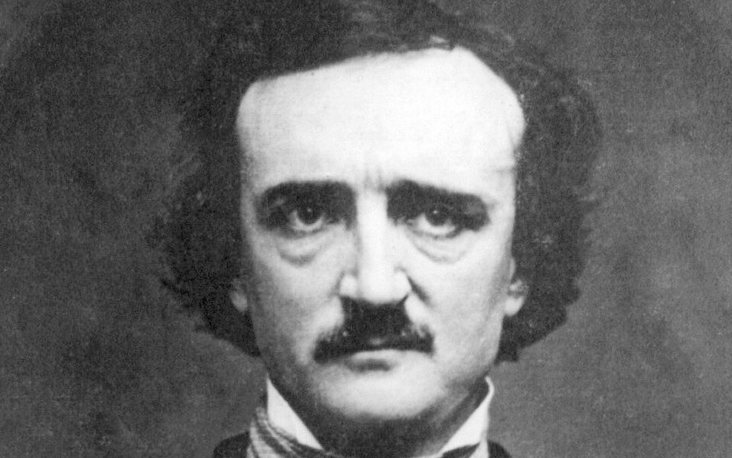
\includegraphics[width=50mm]{images/banner.jpg}
\end{marginfigure}
Ed wrote you a letter containing strange symbols: 
\verb+;85)8( )‡0¶8† -‡*3(5;)+
Can you recover the message?


\hypertarget{HE21.-1}{%
\subsection{HE21.(-1) Solution}\label{he21.-1}}
The image of E. A. Poe directs us towards his cryptography claims,
mainly that he could solve any substitution cipher.  With some guess
work using ``teaser'' as a crib for the first word, we quickly find
the solution \verb+teaser solved congrats+

An alternate approach is to investigate his book ``The golden bug''
where this substitution cipher is taken from.

\hypertarget{HE21.01-first-egg}{%
\section{HE21.01 First egg}\label{HE21.01-first-egg}}

\begin{marginfigure}
    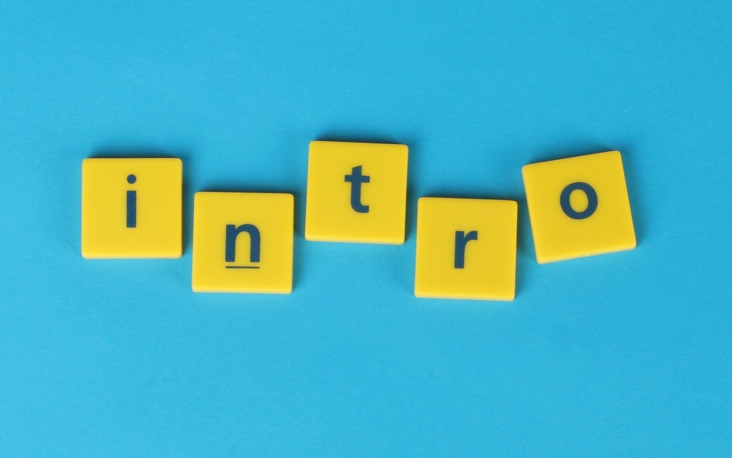
\includegraphics[width=50mm]{images/challenge1.jpg}
\end{marginfigure}
\subsection{Intro}
Well, this is not a real challenge yet, just a quick intro. Some would say sanity check.

\subsection{Event}

\begin{itemize}
  \item The event runs until May 13, 13:37 CET.
  \item Please do not publish write-ups, before that.
  \item There's a Discord server, in case you need support.
\end{itemize}

\subsection{Challenges}

\begin{itemize}
  \item Challenges have difficulty noob, easy, medium, or hard.
  \item Some challenges have a hint - opening the hint is free.
\end{itemize}

\subsection{Flags}

\begin{itemize}
  \item Flag format: \verb+he2021{just_4n_3x4mpl3}+.
  \item There are no flags / eggs hidden in the application - please do not attack it.
\end{itemize}

\subsection{Levels}

\begin{itemize}
  \item With a certain amount of points scored in the current level, you level up.
  \item You can always go back to earlier levels.
  \item That's it for now. Check the HowTo for more details.
\end{itemize}

Time to catch the first flag now! Download the image below.
\begin{marginfigure}
    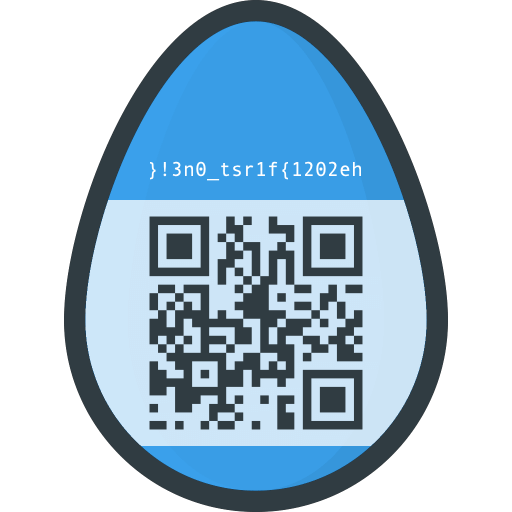
\includegraphics[width=50mm]{ch01/first_egg.png}
%\caption{day01/card.png}
\end{marginfigure}

\hypertarget{he21.01-solution}{%
\subsection{HE21.01 Solution}\label{he21.01-solution}}

Just read the flag backwards.

\hypertarget{he21.02}{%
\section{HE21.02 Basement Cat}\label{he21.02}}

\begin{marginfigure}
    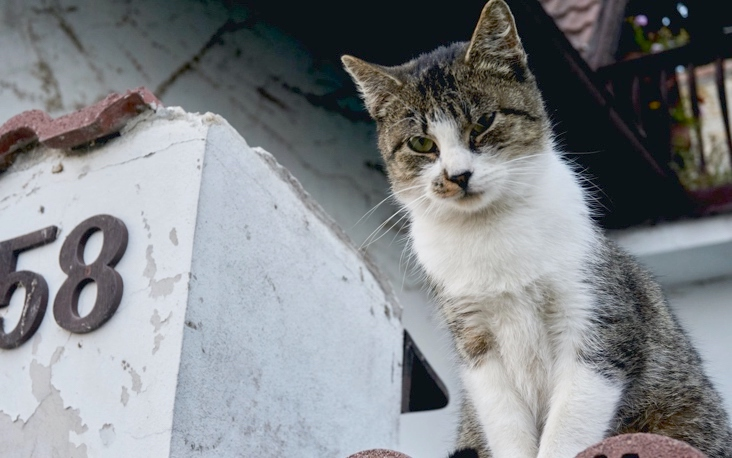
\includegraphics[width=50mm]{images/challenge2.jpg}
\end{marginfigure}
Hi, me iz <strong>Base</strong>ment Cat!

Here iz flag: \verb+5jsnZDgv9EfFeoGXZrFurdz7MWAnK2WaPfszFadr+

\subsection{Show hint (free)}
The number on the image, is a hint! 😉

Check out Cyber Chef.

\hypertarget{he21.02-solution}{%
\subsection{HE21.02 Solution}\label{he21.02-solution}}

The text is base58 encoded, using Cyber Chef it can be converted to
the flag \verb+he2021{meow_nice_to_meet_you}+.

\hypertarget{he21.03}{%
\section{HE21.03 Easy One}\label{he21.03}}

\begin{marginfigure}
    
\includegraphics[width=50mm]{images/challenge3.jpg}
\end{marginfigure}

\noindent How did this happen? This was suppossed to be a
valid QR code, but some ants walked across it. Can you repair the
damage?

\begin{marginfigure}
    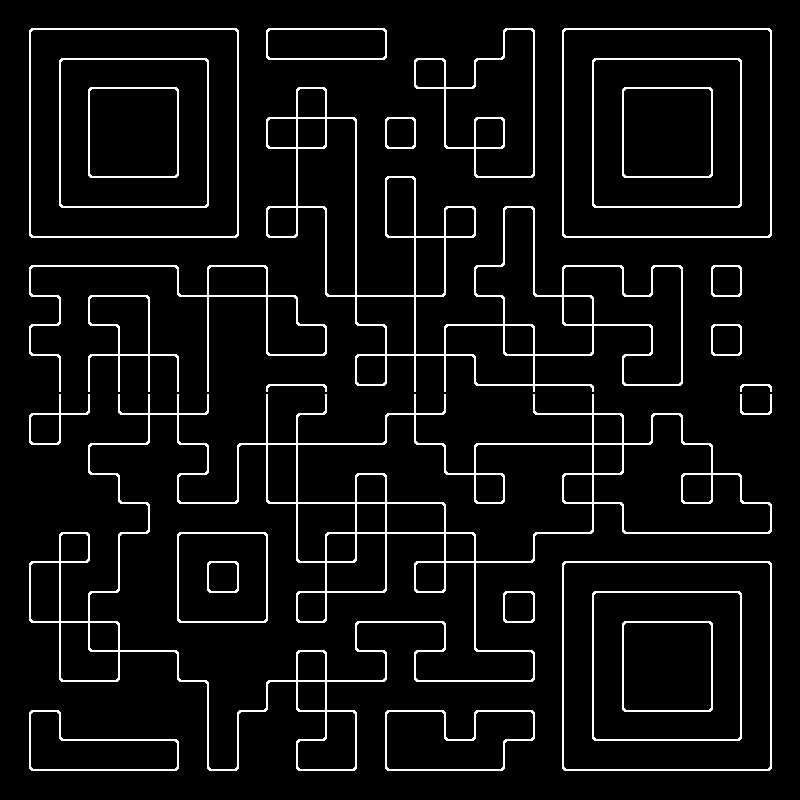
\includegraphics[width=50mm]{ch03/easyone.png}
\end{marginfigure}

\hypertarget{he21.03-solution}{%
\subsection{HE21.03 Solution}\label{he21.03-solution}}

\noindent The file just contains the outline of the QR-code, one line
of pixels is all blacked out, so a fill will have the white bleed into
areas that should be black.  Use Gimp to correct the interrupted white
lines and then start filling with white where appropriate.

\begin{marginfigure}
    
\includegraphics[width=50mm]{ch03/easyone_solved.png}
\end{marginfigure}

\hypertarget{he21.04}{%
  \section{HE21.04 Beehive}
  \label{he21.04}}
% \section{HE21.04 Beehive}

\begin{marginfigure}
    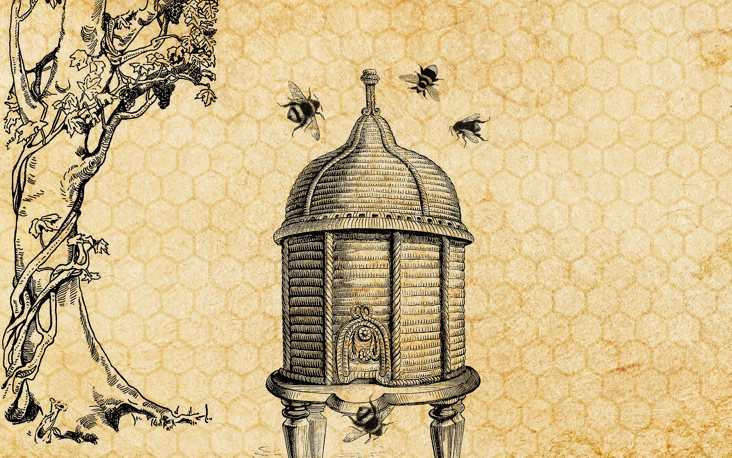
\includegraphics[width=50mm]{images/challenge4.jpg}
\end{marginfigure}


\noindent There's a secret code in the beehive.

⚑ format: he2021{flaglower}.

Lowercase only, and no spaces!
\subsection{Hints}
Kim Godgul

\begin{marginfigure}
    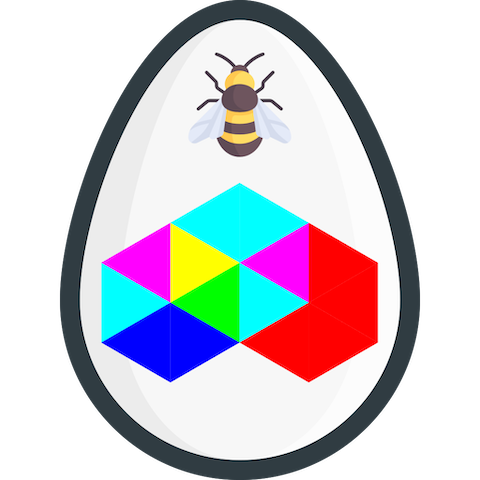
\includegraphics[width=50mm]{ch04/beehive.png}
\end{marginfigure}


\hypertarget{he21.04-solution}{%
\subsection{HE21.04 Solution}\label{he21.04-solution}}

\noindent The hint points us towards some alphabets introduced by Kim
Godgul and we find the
\url{https://omniglot.com/conscripts/colorhoney.php} that shows the
ColorHoney alphabet.  With this we get the flag \verb+he2021{busybee}+

\hypertarget{he21.05}{%
\section{HE21.05 Unicorn}\label{he21.05}}
\begin{marginfigure}
    
\includegraphics[width=50mm]{images/challenge5.jpg}
\end{marginfigure}

\noindent 🦄 Ain't no CTF without a unicorn! 🦄

\begin{verbatim}
s7GvyM1RKEstKs7Mz7NVMtQzUFJIzUvO  
T8nMS7dVCg1x07VQsrfj5bJJzs9LL0os  
KQayFRRs0nIS0+0yUo0MjAyrS/MMkw2K  
8uIN84CiJcbGximKtTb6YBVAffpwjQA=  
\end{verbatim}

\subsection{Show Hint (free)}
Decode and inflate!

\hypertarget{he21.05-solution}{%
\subsection{HE21.05 Solution}\label{he21.05-solution}}

The flag seems to be base64 encoded, so head over to Cyber Chef, but
the result does not resemble anything sensible. So look at the hint
and try to inflate the result and get:

\begin{verbatim}
<?xml version="1.0" encoding="UTF-8"?>
<congrats>
  <flag>he2021{un1c0rn_1nflat333d!}</flag>
</congrats>
\end{verbatim}

\hypertarget{he21.06}{%
  \section{HE21.06 Mystical Symbols}
  \label{he21.06}}
\begin{marginfigure}
    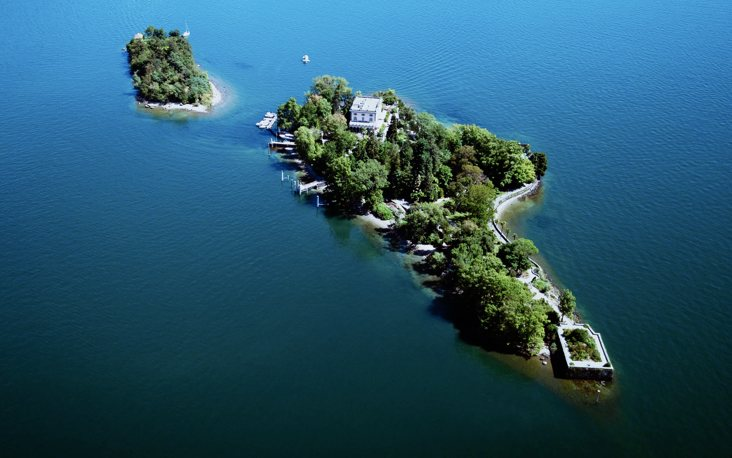
\includegraphics[width=50mm]{images/challenge6.jpg}
\end{marginfigure}

\noindent I found these mystical symbols.

\noindent What do they mean?

\subsection{Show Hint (free)}
\begin{itemize}
\item Really \textbf{myst}ical, isn't it?
\item decimal to ascii
\end{itemize}

\begin{figure}
    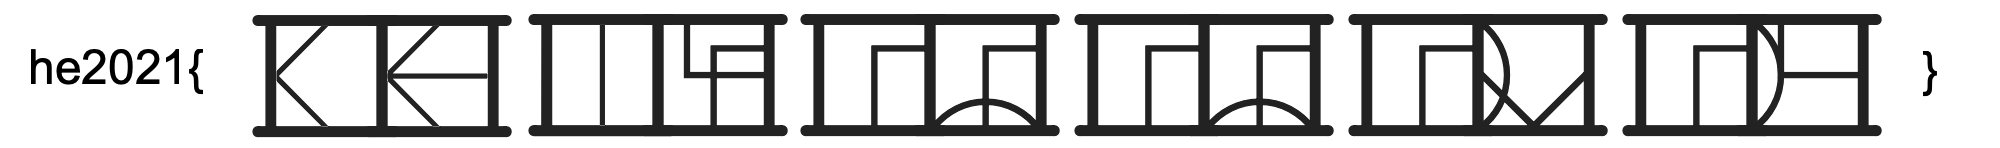
\includegraphics[width=150mm]{ch06/symbols.png}
\end{figure}


\hypertarget{he21.06-solution}{%
\subsection{HE21.06 Solution}\label{he21.06-solution}}

\noindent The symbols looked very familiar, but we could not figure
out where they came from.  The hint then made it clear: the game Myst.
A quick websearch finds
\url{https://dni.fandom.com/wiki/Di\%27ni_Numerals}, which allows us
to translate the symbols into integers: 83, 49, 114, 114, 117, 122

These integers correspond to the ASCII string ``S1rruz'', or the flag \verb+he2021{S1rruz}+.

\hypertarget{he21.07}{%
\section{HE21.07 Caesar's Meme}\label{he21.07}}
\begin{marginfigure}
    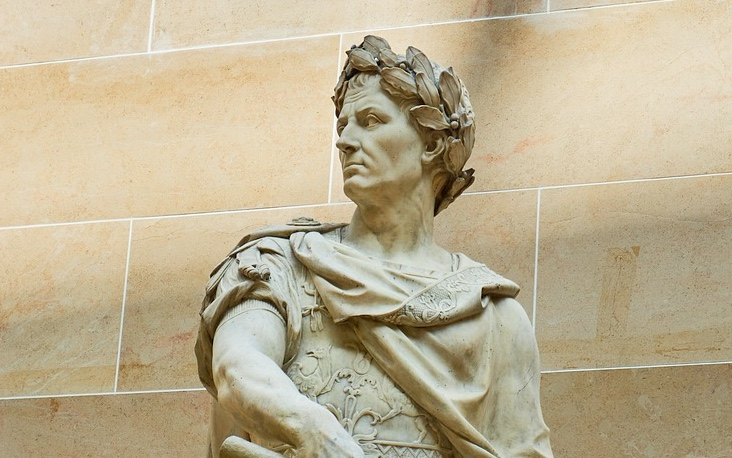
\includegraphics[width=50mm]{images/challenge7.jpg}
\end{marginfigure}

\noindent As is only little known, the ancient Romans invented the memes.

\begin{marginfigure}
    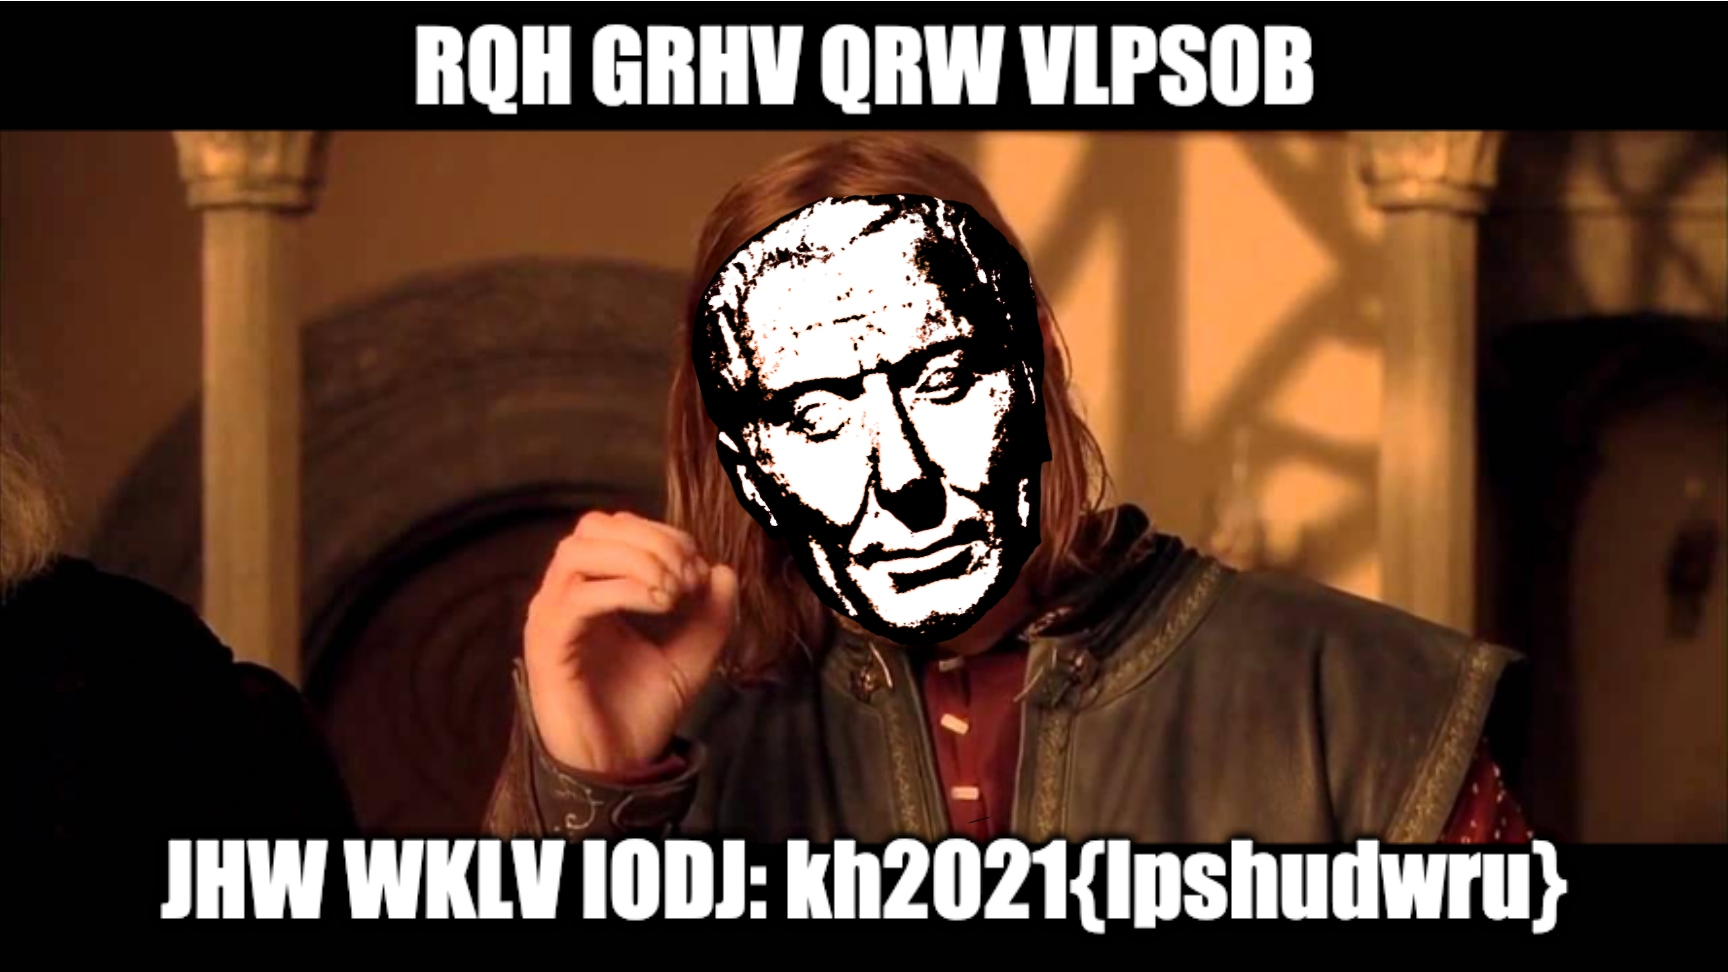
\includegraphics[width=50mm]{ch07/caesarsmeme.jpg}
\end{marginfigure}

\hypertarget{he21.07-solution}{%
\subsection{HE21.07 Solution}\label{he21.07-solution}}

Caesar points towards Ceasar chiffre, so transcribe the text

\verb+RQH GRHV QRW VLPSOB JHW WKLV IODJ: kh2021{lpshudwru}+

into Cyber Chef and play around with the rot parameter.  For a shift
of 23 we get the flag

\verb+ONE DOES NOT SIMPLY GET THIS FLAG: he2021{imperator}+.

\hypertarget{he21.08}{%
\section{HE21.08 Sunshine}\label{he21.08}}
\begin{marginfigure}
    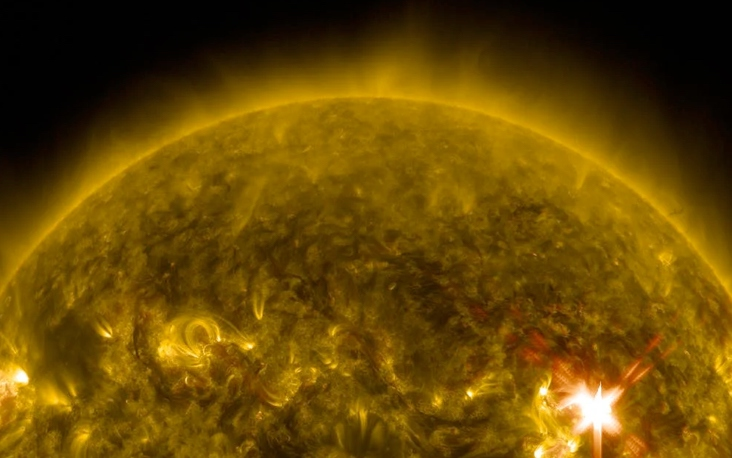
\includegraphics[width=50mm]{images/challenge8.jpg}
\end{marginfigure}

\noindent The rays of sunshine are right there, in front of your eyes.

\begin{marginfigure}
    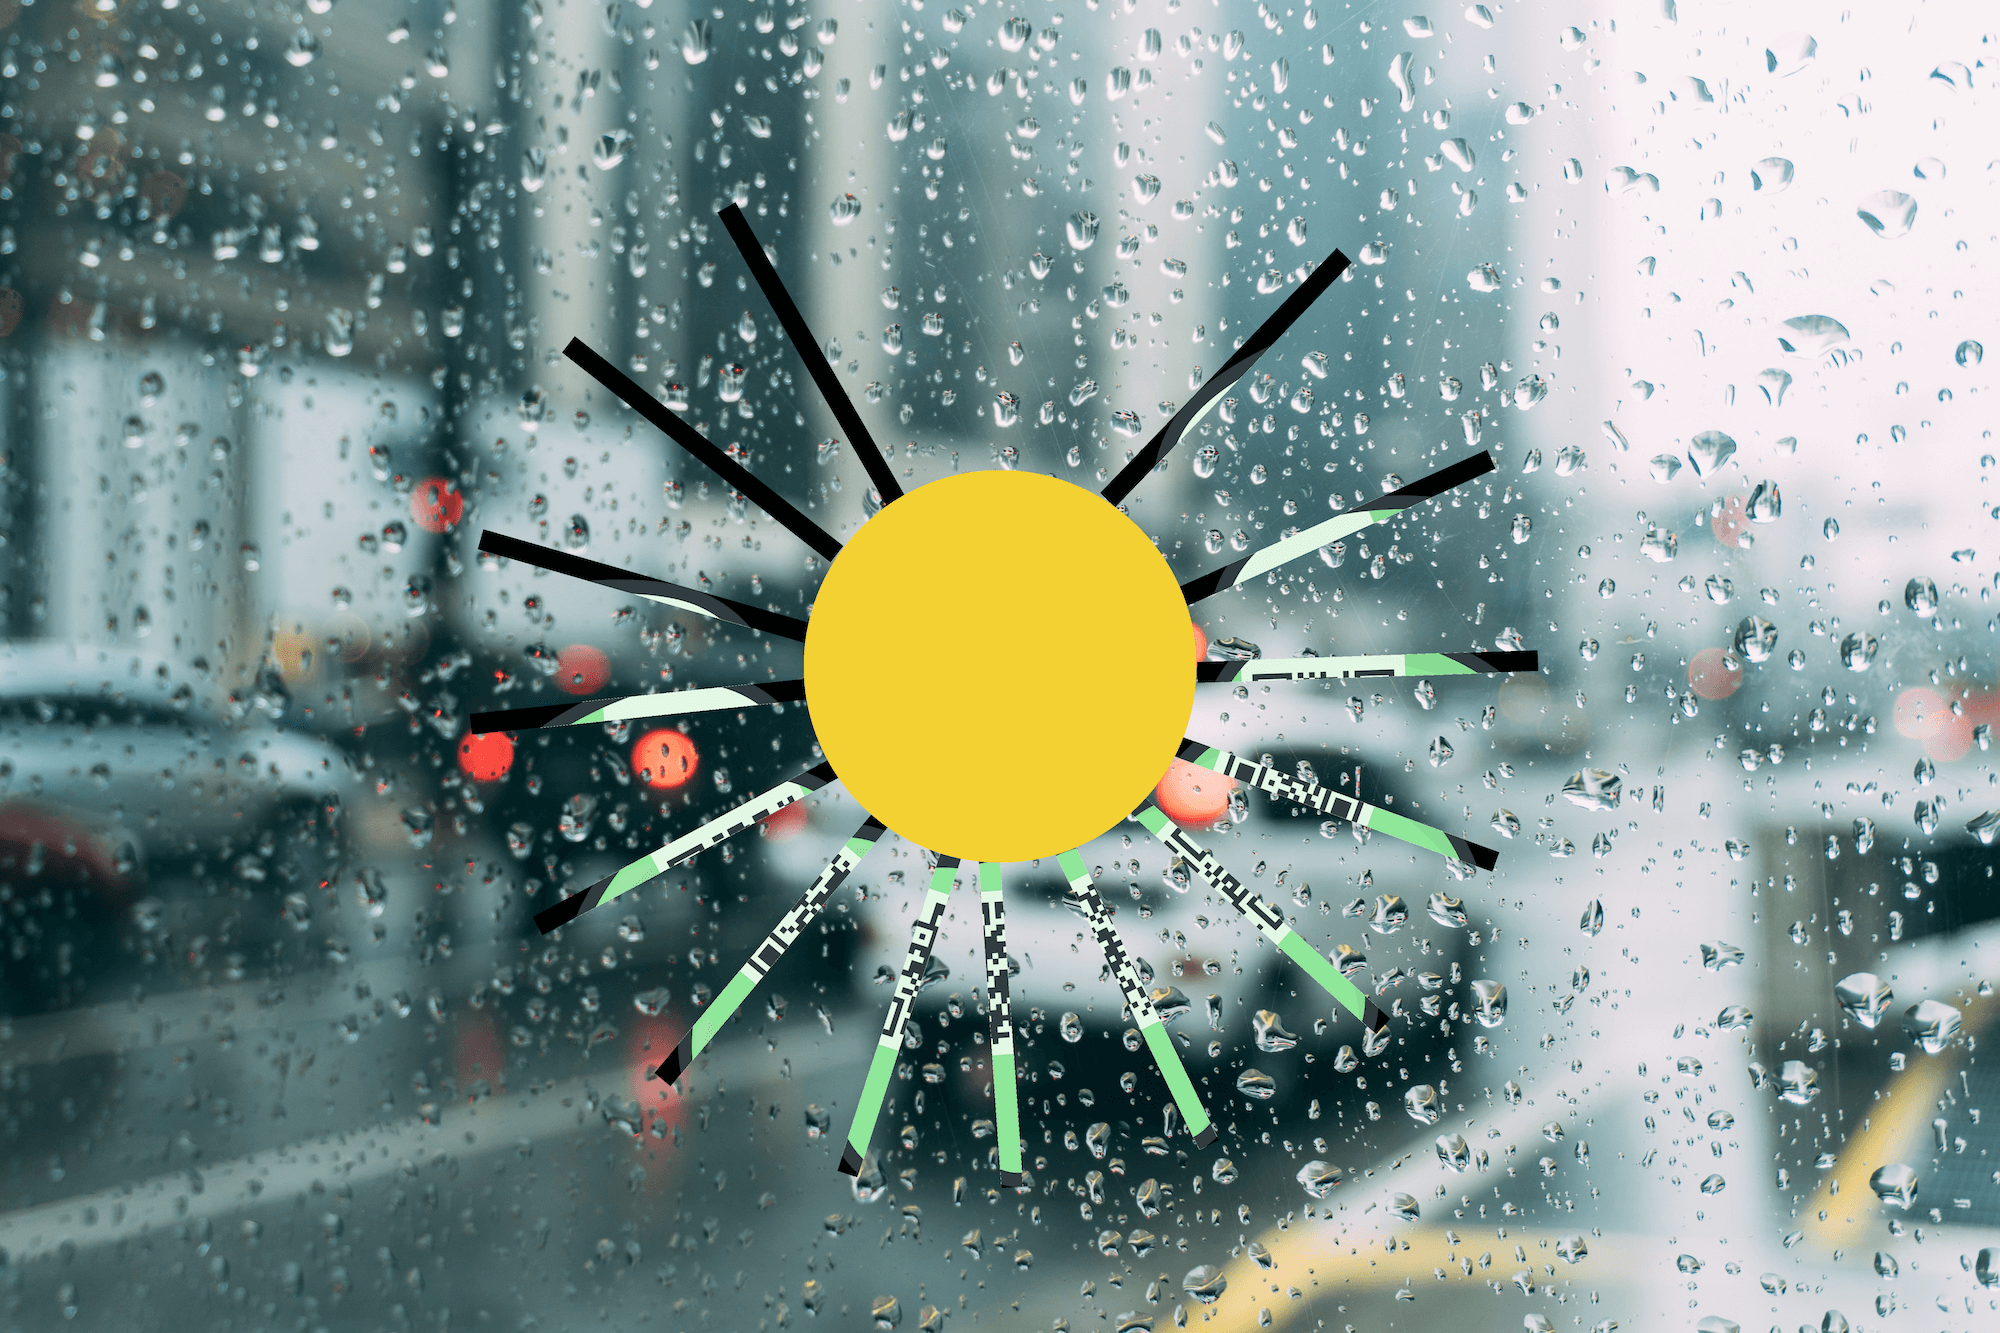
\includegraphics[width=50mm]{ch08/sunshine.png}
\end{marginfigure}

\hypertarget{he21.08-solution}{%
\subsection{HE21.08 Solution}\label{he21.08-solution}}

Use scissors and a steady hand to glue the strips back together. Or find a suitable tool...

\verb+he2021{0h_h3llo_sunsh1ne!}+
\begin{marginfigure}
    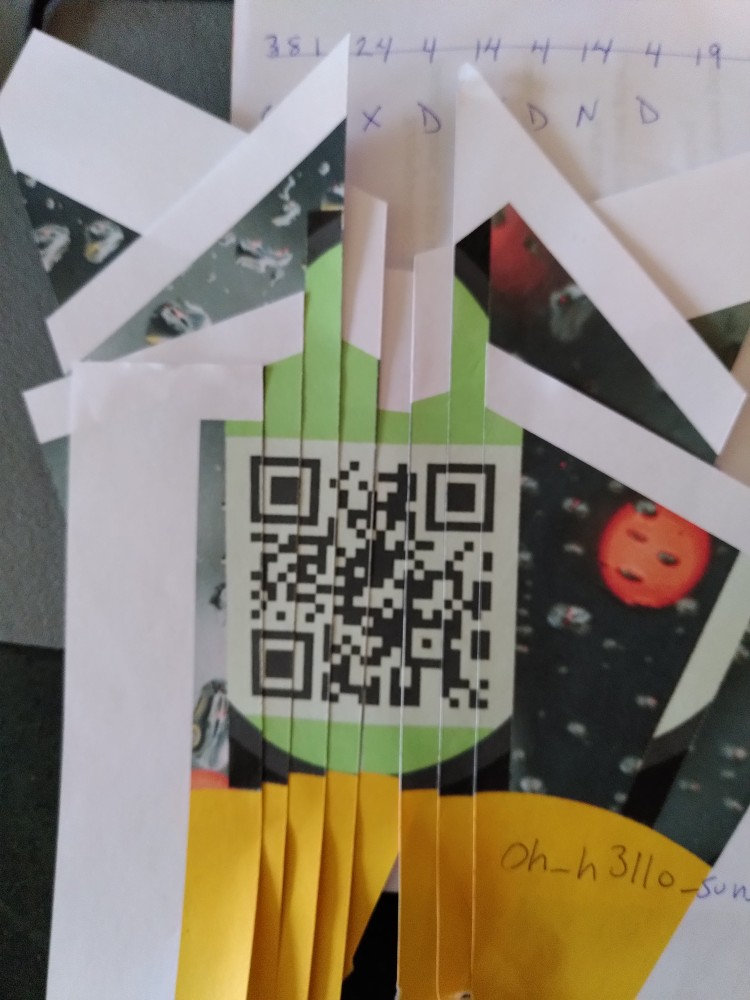
\includegraphics[width=50mm]{ch08/solution08.jpg}
\end{marginfigure}

\hypertarget{he21.09}{%
\section{HE21.09 Cafe Shop}\label{he21.09}}
\begin{marginfigure}
    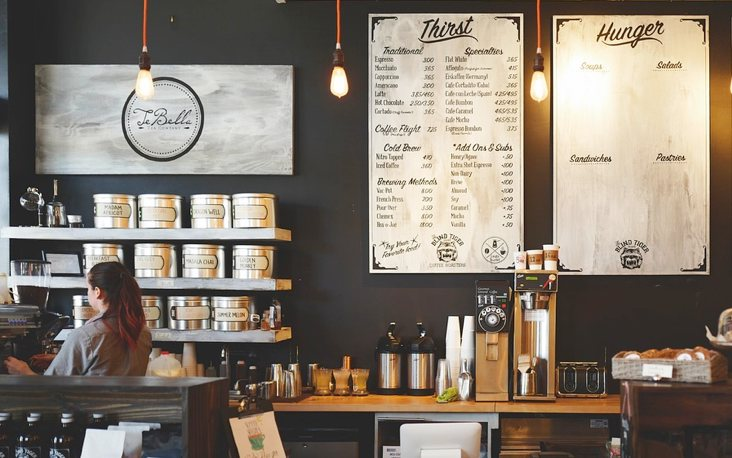
\includegraphics[width=50mm]{images/challenge9.jpg}
\end{marginfigure}

\noindent They have good things at the cafe shop, but I want a COLA - DECAF it must be!

Visit the shop here:
\url{http://46.101.107.117:2104}

Note: The service is restarted every hour at x:00.

\subsection{Show Hint (free)}
\begin{itemize}
\item They also serve hash browns, for \$256.
\end{itemize}

\hypertarget{he21.09-solution}{%
\subsection{HE21.09 Solution}\label{he21.09-solution}}

not yet solved.

Ideas: the hash browns point towards using a hash as a key for the image that is served.

\hypertarget{he21.10}{%
\section{HE21.10 Ghost in a Shell 1}\label{he21.10}}
\begin{marginfigure}
    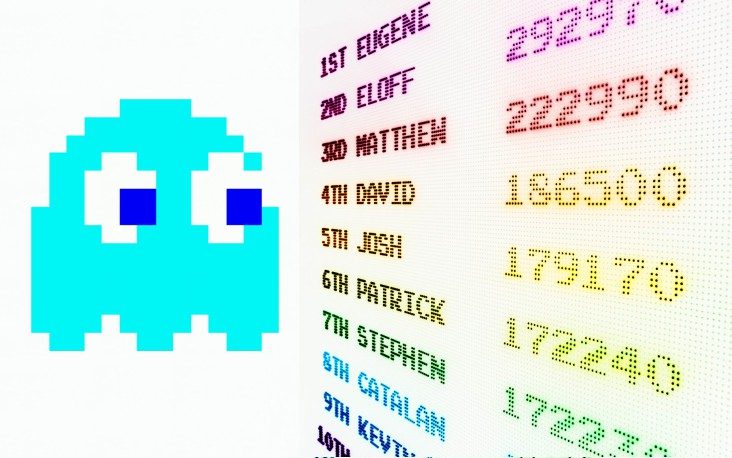
\includegraphics[width=50mm]{images/challenge10.jpg}
\end{marginfigure}

\begin{verbatim}
  _, _,_  _,  _, ___   _ _, _    _,    _, _,_ __, _,  _,    ,  
 / _ |_| / \ (_   |    | |\ |   /_\   (_  |_| |_  |   |     |  
 \ / | | \ / , )  |    | | \|   | |   , ) | | |   | , | ,   |  
  ~  ~ ~  ~   ~   ~    ~ ~  ~   ~ ~    ~  ~ ~ ~~~ ~~~ ~~~   ~  
______________________________________________________________________  
 ,--.    
| oo |   
| ~~ |   o  o  o  o  o  o  o  o  o  o  o  o  o  o  o  o  o  o  o  o  
|/\/\|   
______________________________________________________________________  
\end{verbatim}
Connect to the server, snoop around, and find the flag!

\begin{itemize}
\item \verb+ssh 46.101.107.117 -p 2106 -l inky+
\item password is: \verb+mucky_4444+
\end{itemize}
Note: The service is restarted every hour at x:00.

\hypertarget{he21.10-solution}{%
\subsection{HE21.10 Solution}\label{he21.10-solution}}

Log into the service to find a bunch of files describing the game of
pac-man.  There are two subdirectories, one named ``images'' with a
bunch of pictures, one named ``texts'' with some descriptions of the
adversaries.  Hidden in ``images'' is also a directory named ``...'',
containing a file ``...''.  this file can be copied to the local host
and contains the flag:

\begin{marginfigure}
    
\includegraphics[width=50mm]{ch10/hidden.png}
\end{marginfigure}
\verb+he2021{h1dd3n_d0td0td0t!}+.

\hypertarget{he21.11}{%
\section{HE21.11 Hidden}\label{he21.11}}
\begin{marginfigure}
    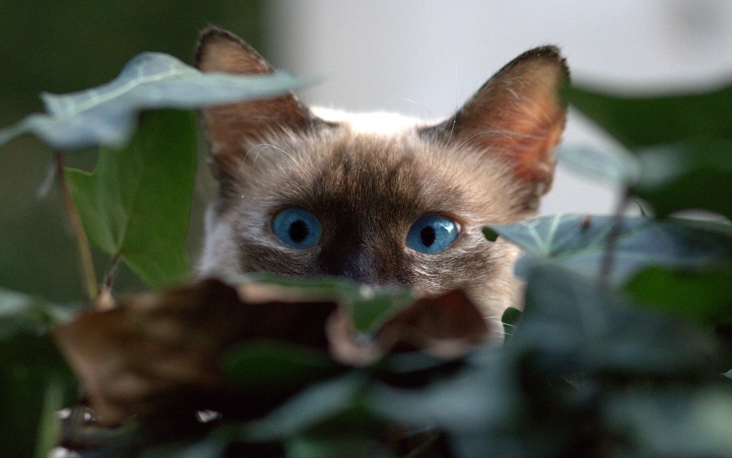
\includegraphics[width=50mm]{images/challenge11.jpg}
\end{marginfigure}

I swear I had the flag a minute ago, but now it seems to be hidden somewhere...

Go back to level 3 and analyze the files of the challenges again. If
you look hard enough, you can find an additional flag.

\subsection{Show Hint (free)}
\begin{itemize}
\item The \textbf{sol}ution is hidden in an image. It's hidden in the
  \textbf{file content}, not in the image (no steganography).
\item There are some numbers in the flag: \verb+he2021{☐☐0☐☐☐☐☐☐☐☐☐☐☐0☐☐☐3☐☐☐☐☐5☐}+
\end{itemize}

\hypertarget{he21.11-solution}{%
\subsection{HE21.11 Solution}\label{he21.11-solution}}
Look into the files of level three. There is one -- sunshine.png --
that matches the hint (in retrospect it is clear what was meant...).
At the end of this PNG file is some ASCII text appended (2800
characters).  If line breaks are inserted every 16 characters, this
pattern emerges:

\begin{verbatim}
0  _              
1 | |__           
2 | '_ \          
3 | | | |         
4 |_| |_|         
5   ___           
6  / _ \          
7 |  __/          
8  \___|          
9  ____           
10 |___ \          
11   __) |         
12  / __/          
13 |_____|         
14   ___           
15  / _ \          
16 | | | |         
17 | |_| |         
18  \___/          
19  ____           
20 |___ \          
21   __) |         
22  / __/          
23 |_____|         
24  _              
25 / |             
26 | |             
27 | |             
28 |_|             
29
\end{verbatim}

Properly transcribed, this gives the flag \verb+he2021{Wh0_is_scared_0f_h3xdump5?}+

And in fact, opening the characters in hexl-mode in Emacs, shows the pattern right away...


\hypertarget{he21.12}{%
\section{HE21.12 Ansi Art}\label{he21.12}}
\begin{marginfigure}
    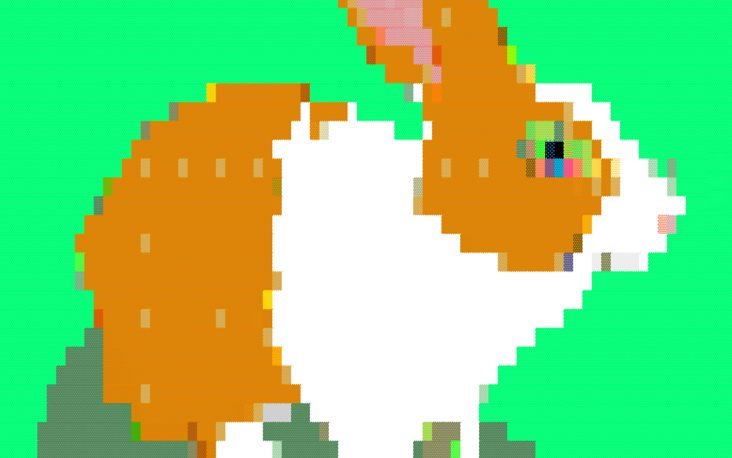
\includegraphics[width=50mm]{images/challenge12.jpg}
\end{marginfigure}

Hope you like my ansi art egg!

Get it with \verb+nc 46.101.107.117 2105+

Note: The service is restarted every hour at x:00.

\hypertarget{he21.11-solution}{%
\subsection{HE21.11 Solution}\label{he21.11-solution}}

Logging into the service spews out a picture of an egg, but with no
writing.  Dumping the output into a file shows that it contains mostly
ANSI terminal control sequences.  Poking around, we find that if we
seach for the letter ``h'', we find a sequence ending with ``h'', then
a sequence ending with ``e'', so this is probably the flag.  Manually
stripping out the control sequences, we get the flag
\verb+he2021{4Ns1MG1k}+


\hypertarget{he21.13}{%
  \section{HE21.13 No No No}
  \label{he21.13}}
\begin{marginfigure}
    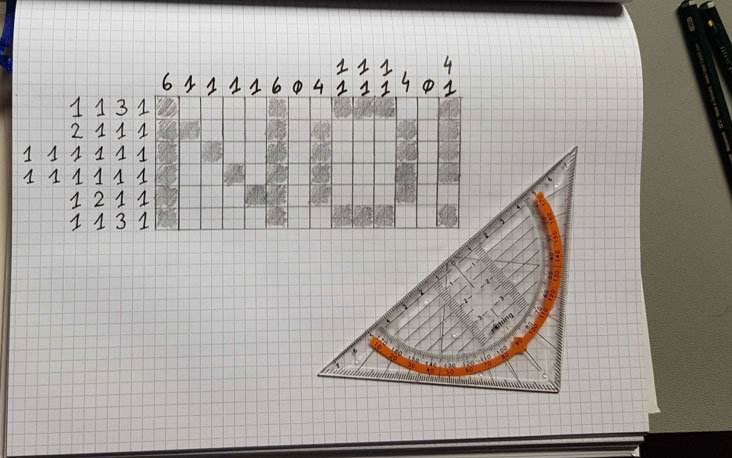
\includegraphics[width=50mm]{images/challenge13.jpg}
\end{marginfigure}

\noindent No! No... nono ..

Where's the egg???

\subsection{Show Hint (free)}
\begin{itemize}
\item Using a tool might be a good idea here.
\item There is a small glitch - if you don't get a solution, try something else.
\end{itemize}

\begin{marginfigure}
    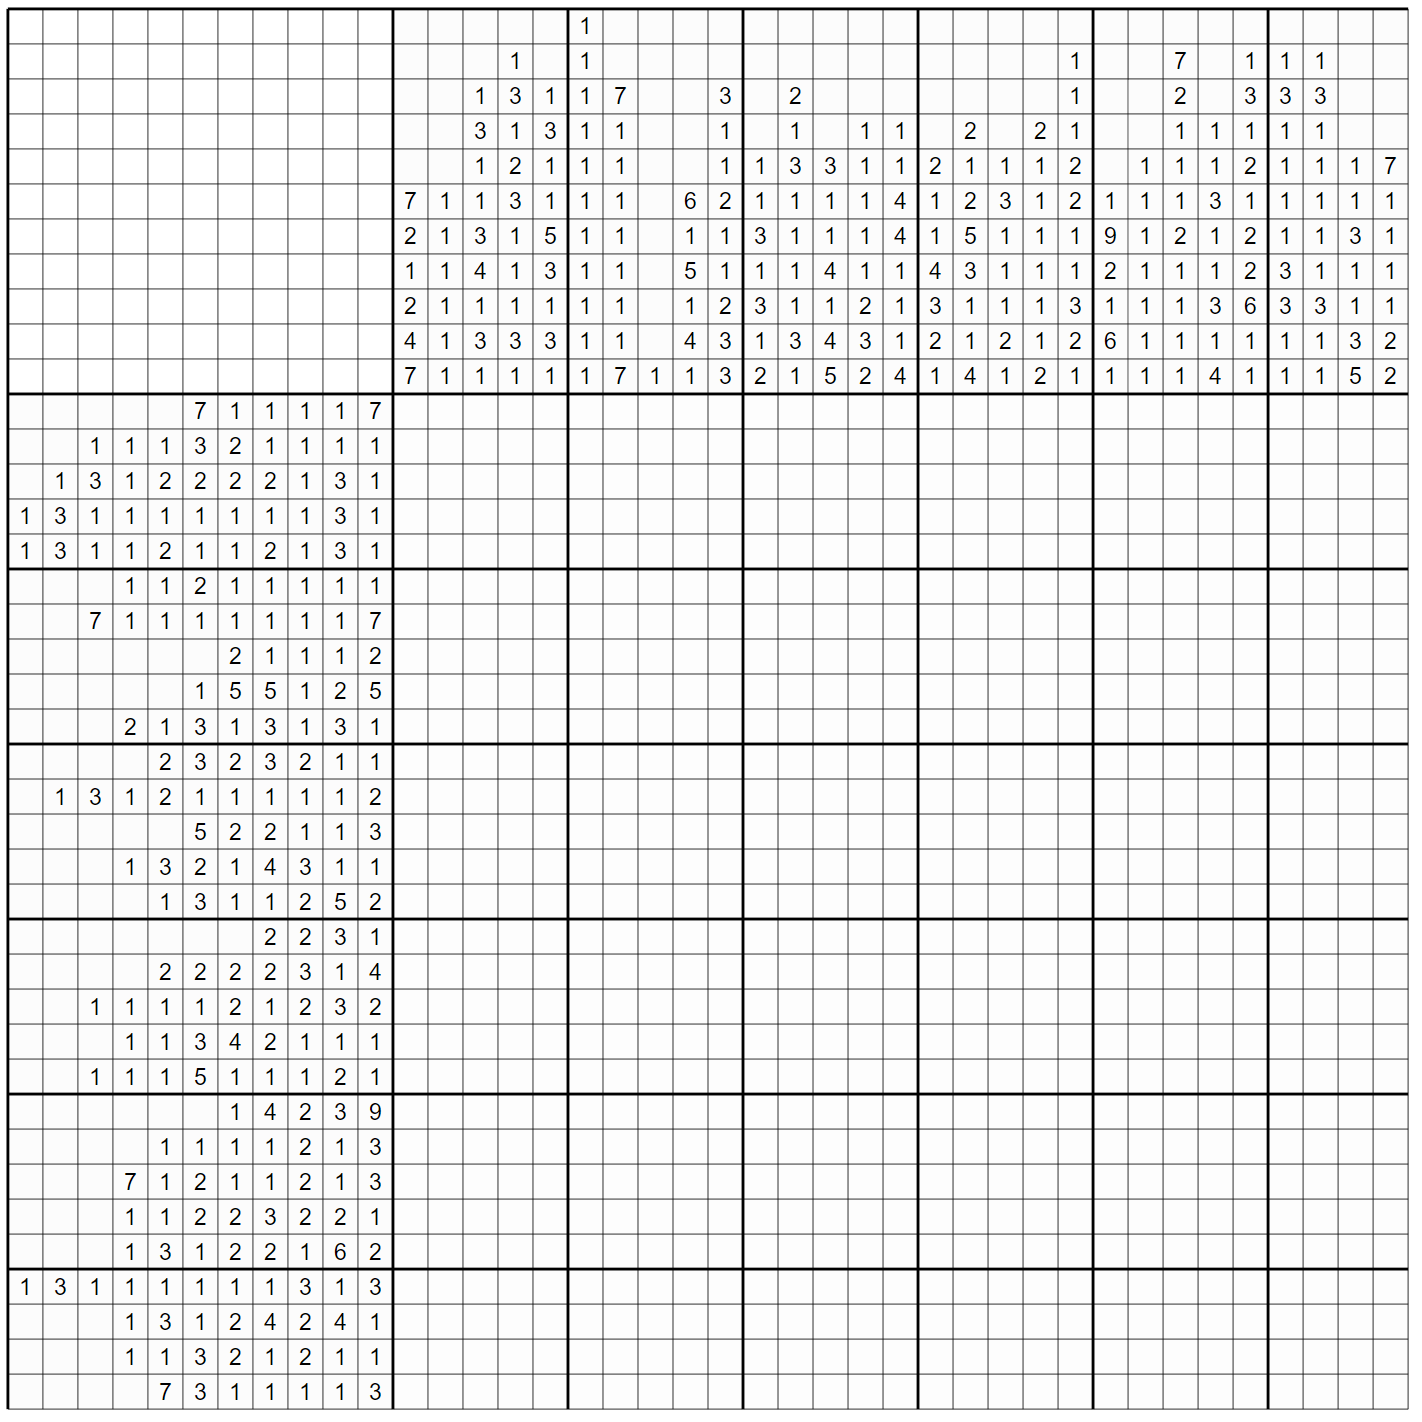
\includegraphics[width=50mm]{ch13/nonobunnygram.png}
\end{marginfigure}


\hypertarget{he21.13-solution}{%
\subsection{HE21.13 Solution}\label{he21.13-solution}}

\noindent The picture shows a nomogram and online there are many
solvers.  We used \url{http://a.teall.info/nonogram}, reading off the
numbers by hand.  The solver does not find a complete solution, but
the error correction of the QR-code is good enough to allow the flag
to be read.

\verb+he2021{Y3sY3sY3sgram_s0unds_a_l0t_nic3r}+.
\begin{figure}
    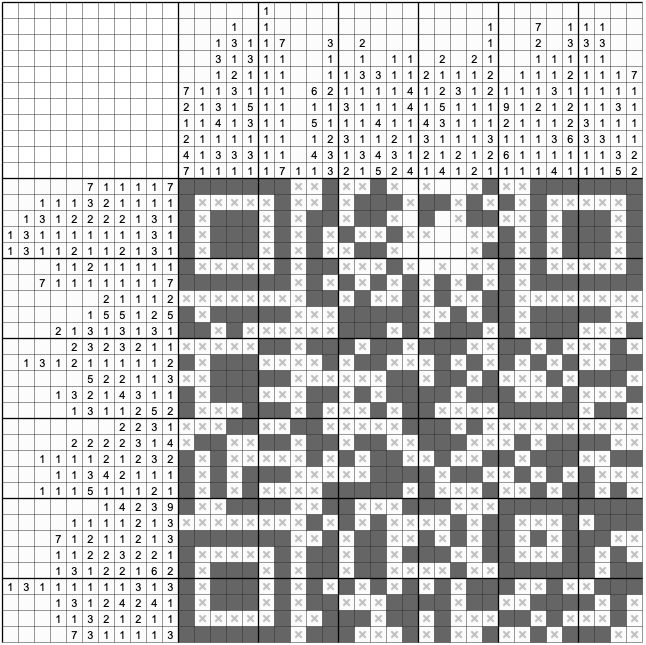
\includegraphics[width=150mm]{ch13/solution13.png}
\end{figure}

\hypertarget{he21.14}{%
  \section{HE21.14 Haxxor what?}
  \label{he21.14}}
\begin{marginfigure}
    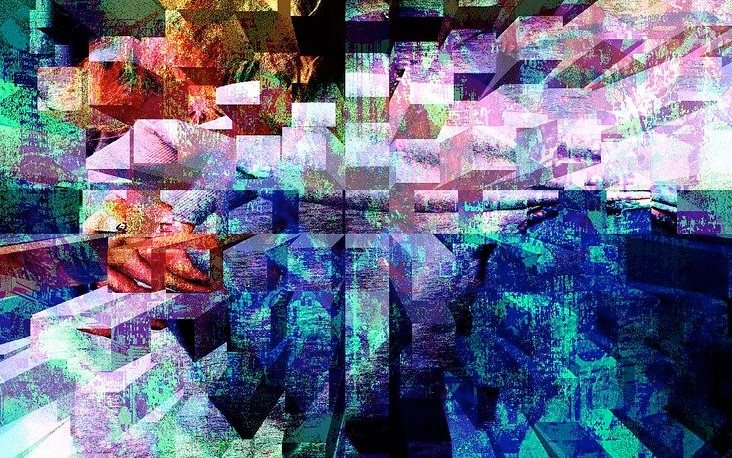
\includegraphics[width=50mm]{images/challenge14.jpg}
\end{marginfigure}

\noindent I got this image of an Easter egg.

But what kind of encryption is this?!

\subsection{Show Hint (free)}
\begin{itemize}
\item The original file is an image
\end{itemize}


\hypertarget{he21.14-solution}{%
\subsection{HE21.14 Solution}\label{he21.14-solution}}

\noindent The file is a binary file, from the hint and the title we assume that it is XOR'ed with a constant key.  Assuming a PNG file, we can use the first few bytes as a crypt and get the key:
\begin{itemize}
\item See \url{http://libpng.org/pub/png/spec/1.2/PNG-Structure.html} for the file signature (decimal): 137 80 78 71 13 10 26 10
  
\item Use Cyber Chef to XOR this signature with the file to get this key: \verb+haxxors!+
\end{itemize}

Then XOR the file using \verb+xortools-xor+

\begin{verbatim}
% xortool-xor -r 'haxxors!' -f haxxorwhat  >output.png 
\end{verbatim}

to get the egg and the flag
\verb+he2021{r34l_x0r_h4xx0r}+.
\begin{marginfigure}
    
\includegraphics[width=50mm]{ch14/output.png}
\end{marginfigure}

\hypertarget{he21.15}{%
  \section{HE21.15 Social Checker}
  \label{he21.15}}
\begin{marginfigure}
    
\includegraphics[width=50mm]{images/challenge15.jpg}
\end{marginfigure}

\noindent Social Checker - check if your favourite social media site is online!

\url{http://46.101.107.117:2103}

Note: The service is restarted every hour at x:00.

\subsection{Show Hint (free)}
\begin{itemize}
\item Some characters are blocked - find a workaround!
\end{itemize}


\hypertarget{he21.15-solution}{%
\subsection{HE21.15 Solution}\label{he21.15-solution}}

\noindent 

\hypertarget{he21.16}{%
  \section{HE21.16 LOTL}
  \label{he21.16}}
\begin{marginfigure}
    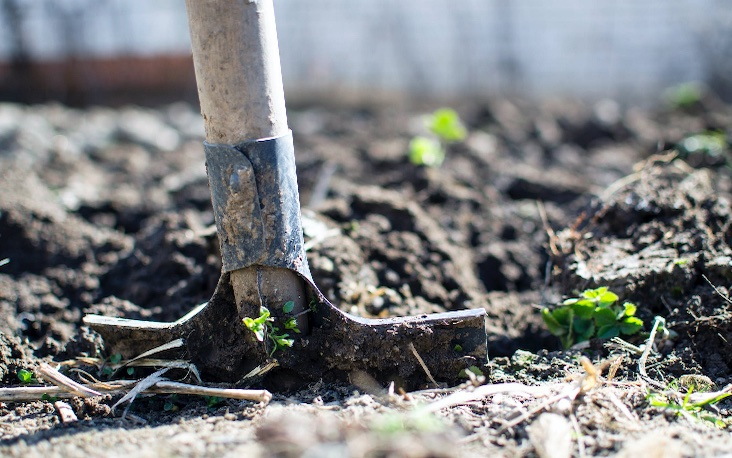
\includegraphics[width=50mm]{images/challenge16.jpg}
\end{marginfigure}

\noindent Save the planet!

Well, we should then better LOTL and use what we have, right?

\verb+nc 46.101.107.117 2102+

Get a shell and read the flag.

Note: The service is restarted every hour at x:00.

Executable ``lotl'' is provided.

\hypertarget{he21.16-solution}{%
\subsection{HE21.16 Solution}\label{he21.16-solution}}

\noindent 

\hypertarget{he21.17}{%
  \section{HE21.17 Digizzled}
  \label{he21.17}}
\begin{marginfigure}
    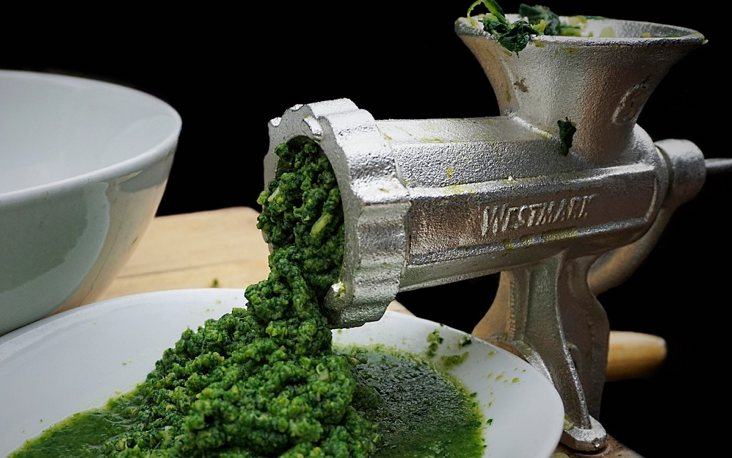
\includegraphics[width=50mm]{images/challenge17.jpg}
\end{marginfigure}

\noindent Had a flag, but it got digizzled. Can you recover it?

\begin{verbatim}
-------------------------------------  
      o                  o             
      | o      o         |             
    o-O   o--o   o-o o-o | o-o o-o     
   |  | | |  | |  /   /  | |-' |       
    o-o | o--O | o-o o-o o o-o o       
             |                         
         o--o                          
-------------------------------------
enter flag: [REDACTED]    
digizzling...  
c5ab05ca73f205ca  
\end{verbatim}

A file ``digizzle'' is given.

\hypertarget{he21.17-solution}{%
\subsection{HE21.17 Solution}\label{he21.17-solution}}

\noindent The file is a dump of disassembled python code; check the
documentation on the module \verb+dis+.  If python 3.7 is used, the
disassembly can be reproduced by this code:

\begin{minted}{python}
import re
pattern = re.compile('^he2021\\{([dlsz134]){9}\\}$')

def hizzle(s):
    s1 = 13
    s2 = 37
    for n in range(len(s)):
        s1 = (s1 + ord(s[n])) % 65521
        s2 = (s1 * s2) % 65521
    return (s2 << 16) | s1

def smizzle (a,b):
    return format(a, 'x') + format(b, 'x')

print('-------------------------------------')
print('      o                  o           ')
print('      | o      o         |           ')
print('    o-O   o--o   o-o o-o | o-o o-o   ')
print("   |  | | |  | |  /   /  | |-' |     ")
print('    o-o | o--O | o-o o-o o o-o o     ')
print('             |                       ')
print('         o--o                        ')
print('-------------------------------------')
s = input('enter flag:')
res = pattern.match(s)
if res:
    print('digizzling...')
    a = hizzle(s)
    b = hizzle(s[::-1])

    print(smizzle(a,b))

else:
    print('wrong format!')  
  \end{minted}

  We know the expected result for the flag and build a brute forcing
  loop.  Since the function \verb+smizzle+ does only a conversion from
  integer to string and then a string concatenation, we can leave it
  away and compare directly with integers.

  \begin{minted}{python}
    alph = 'dlsz134'
    
    for c1 in alph:
    for c2 in alph:
    print(c2)
    for c3 in alph:
            for c4 in alph:
                for c5 in alph:
                    for c6 in alph:
                        for c7 in alph:
                            for c8 in alph:
                                for c9 in alph:
                                    s = 'he2021{' + c1 + c2 + c3+ c4 + c5 + c6+ c7 + c8 + c9 + '}'
                                    a = hizzle(s)
                                    if a == 0xc5ab05ca:
                                        b = hizzle(s[::-1])
                                        if b == 0x73f205ca:
                                            print(s)
                                            print(smizzle(a,b))
                                            sys.exit(0)
  
  \end{minted}

The flag is \verb+he2021{d1s4zzl3d}+

\hypertarget{he21.18}{%
  \section{HE21.18 Bunny Beat}
  \label{he21.18}}
\begin{marginfigure}
    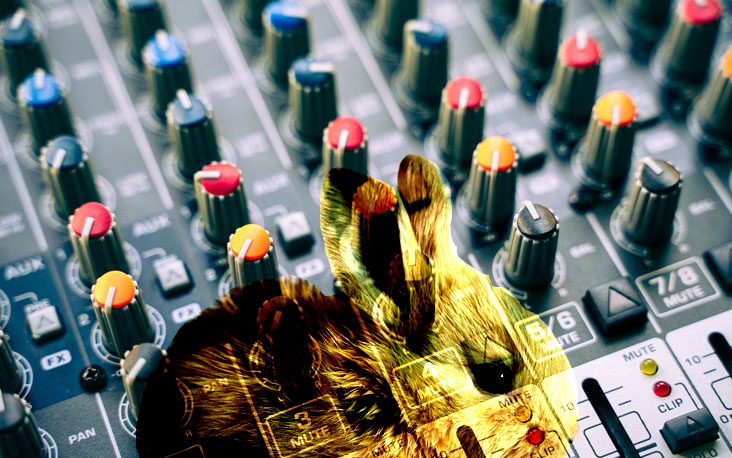
\includegraphics[width=50mm]{images/challenge18.jpg}
\end{marginfigure}

\noindent The bunnies have discovered minimal beats!

But where is the flag?

Wave file \verb+bunnybeat.wav+ is given.

\hypertarget{he21.18-solution}{%
\subsection{HE21.18 Solution}\label{he21.18-solution}}

\noindent Look at the wave file in Sonic Visualiser and check out the
spectrogram.  Then the flag stands out immediately
\verb+he2021{Sp3ctrogramsROCK!}+.

\begin{marginfigure}
    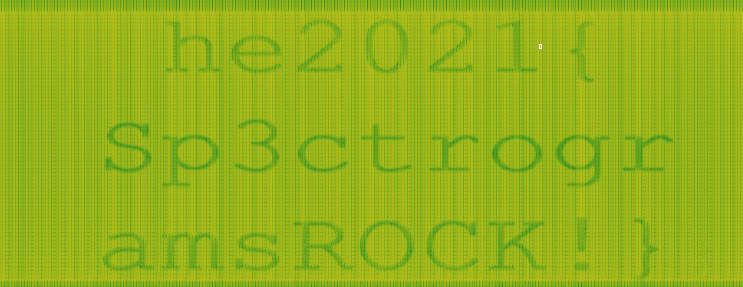
\includegraphics[width=50mm]{ch18/spectrogram.png}
\end{marginfigure}


\hypertarget{he21.19}{%
  \section{HE21.19 😈}
  \label{he21.19}}
\begin{marginfigure}
    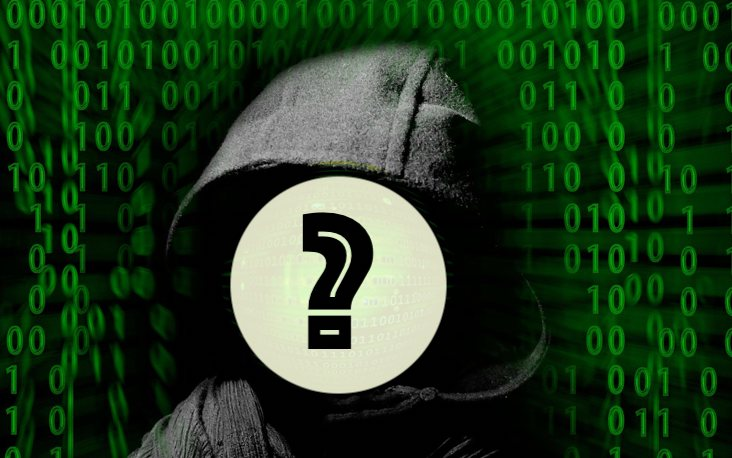
\includegraphics[width=50mm]{images/challenge19.jpg}
\end{marginfigure}

\noindent One of the bunnies made a new friend. But when asked for the name, he only got the response below.

Can you find out the friend's name, in UPPERCASE?

\begin{verbatim*}
▫️▫️😈😈▫️▫️▫️😈▫️▫️😈😈▫️▫️▫️▫️▫️▫️😈😈▫️▫️▫️▫️▫️▫️😈😈▫️▫️▫️▫️▫️▫️😈😈▫️▫️▫️▫️▫️▫️😈😈▫️▫️▫️▫️▫️▫️😈😈▫️▫️▫️▫️▫️▫️😈😈▫️▫️▫️▫️▫️▫️😈😈▫️▫️▫️▫️▫️▫️😈😈▫️▫️▫️▫️▫️▫️😈😈▫️▫️▫️▫️▫️▫️😈😈▫️▫️▫️▫️▫️▫️😈😈▫️▫️▫️▫️▫️▫️😈😈▫️▫️▫️▫️▫️▫️😈😈▫️😈😈▫️▫️▫️😈😈▫️😈😈▫️▫️▫️😈😈▫️😈😈▫️▫️▫️😈😈▫️▫️▫️▫️▫️▫️😈😈▫️▫️▫️▫️▫️▫️😈😈▫️▫️▫️▫️▫️▫️😈😈▫️▫️▫️▫️▫️▫️😈😈▫️▫️▫️▫️▫️▫️😈😈▫️▫️▫️▫️▫️▫️😈😈▫️▫️▫️▫️▫️▫️😈😈▫️▫️▫️▫️▫️▫️😈😈▫️▫️▫️▫️▫️▫️😈😈▫️▫️▫️▫️▫️▫️😈😈▫️▫️▫️▫️▫️▫️😈😈▫️▫️▫️▫️▫️▫️😈😈▫️▫️▫️▫️▫️▫️😈😈▫️▫️▫️😈
\end{verbatim*}

⚑ format: \verb+he2021{JOHNDOE}+

\subsection{Show Hint (free)}
\begin{itemize}
\item We need the name of what you find, in UPPERCASE, and wrapped in he2021{...}.
\end{itemize}


\hypertarget{he21.19-solution}{%
\subsection{HE21.19 Solution}\label{he21.19-solution}}

\noindent This was supposed to be easy, but it took us longer than
many others so far.  The input string contains two symbols that can be
translated to a binary representation and, when chopped into 8 bit
pieces, interpreted as characters.  This gives us a string
\verb+1000000000000066600000000000001+.  After many futile attempts,
we found that it is called ``Belphegor's prime'' and so the flag is
\verb+he2021{BELPHEGOR}+.

\hypertarget{he21.20}{%
  \section{HE21.20 Run Me, Baby!}
  \label{he21.20}}
\begin{marginfigure}
    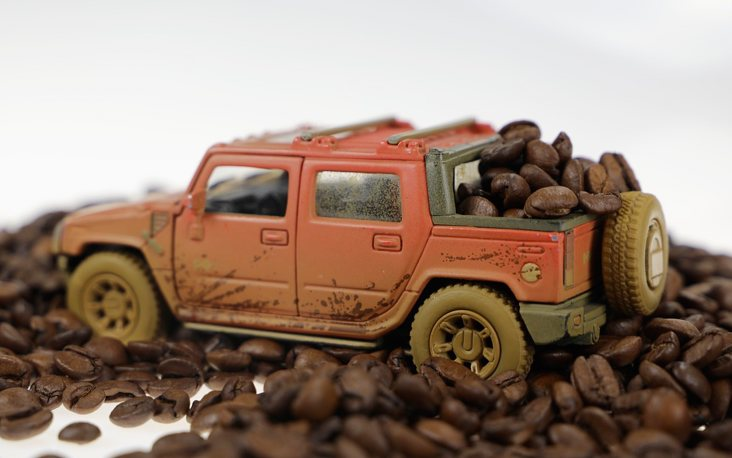
\includegraphics[width=50mm]{images/challenge20.jpg}
\end{marginfigure}

\noindent This one's easy, ain't it? Just run the .class file. Hope you like Java!

Class file \verb+runme.class+ is given.

\hypertarget{he21.20-solution}{%
\subsection{HE21.20 Solution}\label{he21.20-solution}}

\noindent The class file is not from a Java program, but from a Groovy
program.  Decompiling the class file using cfr gave a quite convoluted
java file.  Since the challenge is labelled as easy, we tried to run
the Groogy program directly.  But when we failed, we quickly re-wrote
it in python to get the flag \verb+he2021{isnt_17_gr00vy_baby?}+

\begin{minted}{python}
s = [1, 6, 7, 3, 2, 9, 4, 5, 3, 4, 8, 9, 1, 7, 3, 2, 3, 3, 7, 8, 7, 3, 2, 4, 5, 3, 5, 1, 3, 0, 3, 4, 5, 5]
cipher = "ik934:\u007fnvr|h2>biu37~\u0080bdeg|D~"
sol = ''

for i in range(len(cipher)):
    t = ord(cipher[i]) - s[i]
    sol += chr(t)
print(sol)
\end{minted}

\hypertarget{he21.21}{%
  \section{HE21.21 Memeory 3.0 -- The Finale}
  \label{he21.21}}
\begin{marginfigure}
    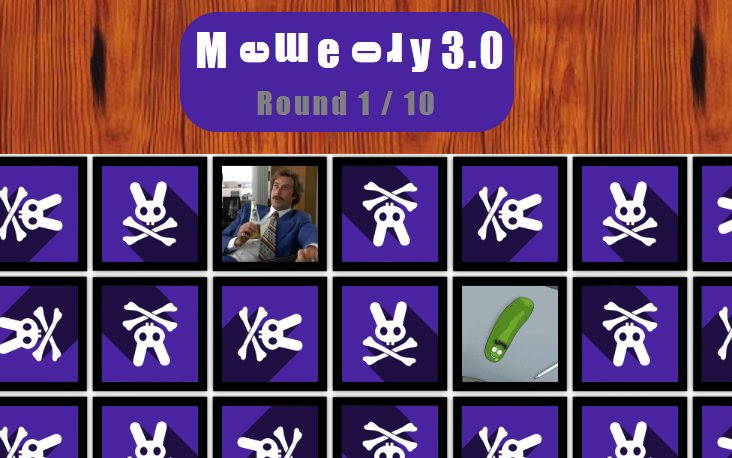
\includegraphics[width=50mm]{images/challenge21.jpg}
\end{marginfigure}

\noindent We finally fixed Memeory 2.0 and proudly release Memeory 3.0 aka the supersecure-Memeory.

Flagbounty for everyone who can solve 10 successive rounds. Time per round is 30 seconds and only 3 missclicks are allowed.

\url{http://46.101.107.117:2107}

Note: The service is restarted every hour at x:00.
Class file \verb+runme.class+ is given.

\hypertarget{he21.21-solution}{%
\subsection{HE21.21 Solution}\label{he21.21-solution}}

\noindent This is an extension of an older challenge: play memory on-line.  The
path to solve it remains the same: load all images (labelled from 1 to 98),
identify which ones are the same and the post the proper pairs.  Compared to
the last installment, the images can be rotated and so we have to identify
them.  This is a similar task as in HackyEaster 2019, 'Egg CAPTCHA'.  Basically
write some code to compare all possible orientation of a picture with another
picture and calculate a figure of merit.  I chose an rms distance and this
worked well:

\begin{minted}{python}
import requests
import numpy as np
from PIL import Image


def mse(im1_arr, im2_arr):
    #diff = im1_arr - im2_arr
    err = np.sum((im1_arr - im2_arr) ** 2)
    err /= float(im1_arr.shape[0])
    return 3.0*err

def match(im1_arr, im2_arrs):
    rms = np.empty(4, dtype=np.float)
    for i in range(4):
        rms[i] = mse(im1_arr, im2_arrs[i])
    avg = np.sum(rms) / 4.0
    rms2 = np.true_divide(rms, avg)
    return (np.max(rms2) - np.min(rms2))

def match_with(im, im2, thresh):
    (sX,sY) = im.size
    arrlen = sX*sY*3
    (sX2,sY2) = im2.size

    if sX == sX2 and sX == sY2 and sX == sY:
        # build an array with all rotated images as arrays
        im_arrs = []
        for i in range(4):
            im_arrs.append(np.array(im, dtype=np.float).reshape((arrlen)))
            if i < 3:
                im = im.rotate(90)
        im_arr2 = np.array(im2, dtype=np.float).reshape((arrlen))
        m = match(im_arr2,im_arrs)
        if m > thresh:
            return True
    else:
        if sX == sX2 and sY == sY2:
            return True
        elif sX == sY2 and sY == sX2:
            return True
        else:
            return False
    return False
\end{minted}

The code is straight-forward, the only issue was with images that are not
square: these cannot be dealt with so easily; for now we just assume that they
are the same, if the dimensions are compatible.

Solving the challenge is then relatively easy:
\begin{minted}{python}
base_url = "http://46.101.107.117:2107/"
def getPics(s):
    pics = {}
    for i in range(1,99):
        u = base_url+'pic/%d'%i
        r = s.get(u)
        with io.BytesIO(r.content) as imgF:
            img = Image.open(imgF)
            img.load()
            pics[i] = img
    return(pics)


def runMatch(session, pics, found, thresh):
    solve_url = base_url+'solve'
    post_data = {'first': '1', 'second': '2'}
    for i in range(1,99):
        if not found[i]:
            for j in range(i+1, 99):
                if not found[j]:
                    try:
                        if match_with(pics[i], pics[j], thresh):
                            post_data['first'] = i
                            post_data['second'] = j
                            r = session.post(solve_url, post_data)
                            if r.text[:2] != 'ok' and r.text != 'nextRound':
                                raise ValueError
                            # print('pics %d and %d match!' %(i,j))
                            found[i] = True
                            found[j] = True
                            break
                    except ValueError:
                        print(i,j)
                        print(pics[i].size, pics[j].size)
                        print(r.text)
                        # pics[i].show()
                        # pics[j].show()
                        pass

    nNotFound = 0
    for v in found:
        if not v:
            nNotFound += 1
    return r.text, session, found, nNotFound

def solveRound(session):
    r = session.get(base_url)
    pics = getPics(session)
    found = [False for i in range(99)]
    found[0] = True
    nNotFound = 98
    thresh = 0.9

    while nNotFound > 0:
        result, session, found, nNotFound = \
            runMatch(session, pics, found, thresh)
        print(result, nNotFound, thresh)
        thresh -= 0.1
    return result


def solve():
    count = 0
    ok = 'nextRound'
    res = ok
    session = requests.session()
    while res == ok:
        count += 1
        print('round: ', count)
        res = solveRound(session)
        print(res)


solve()
\end{minted} 

In the end we get the result
\verb+ok, here is your flag: he2021{0k-1-5u44end3r-y0u-w1n!}+
and the flag \verb+he2021{isnt_17_gr00vy_baby?}+


\hypertarget{he21.22}{%
  \section{HE21.22 46 Apes}
  \label{he21.22}}
\begin{marginfigure}
    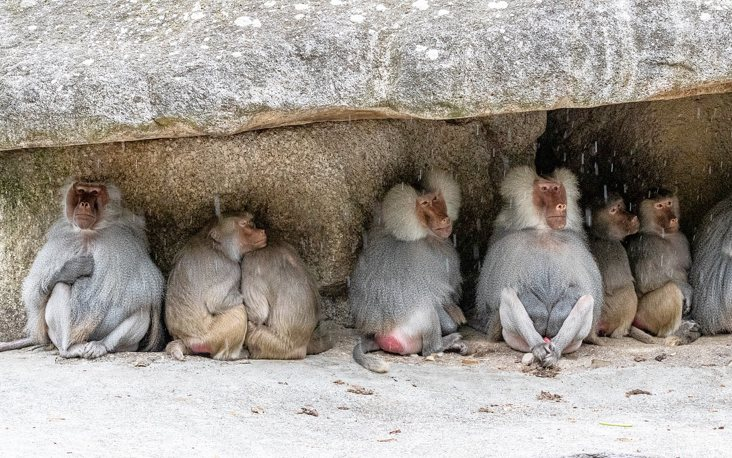
\includegraphics[width=50mm]{images/challenge22.jpg}
\end{marginfigure}

\noindent 46 apes encoded a message for you:

\verb+2Qu93ZhJHdsMGIlhmcgUXagMWe19icmBGbnFiOoBTZwIjM7FGd0gHdfNTbuB2a5V2X1JzcuF3MzNQf==+

\hypertarget{he21.22-solution}{%
\subsection{HE21.22 Solution}\label{he21.22-solution}}

\noindent First thought: it looks like base64 encoded, but this yields a binary.  But ``46 Apes'' could mean to reverse the string, except for the padding.  So head over to Cyber Chef and try: \verb+}.s3qns2u_eyk`nm3_tx4ta{220e0h:!gl`fr/uyc iu rhe c,trag.nC+. This looks much better, as it is all printable characters and it is kind of reversed.  The last word is probably ``Congrats'', so see what is up:

\begin{verbatim}
>>> base64.b64encode(b'Congrats')
b'Q29uZ3JhdHM='
\end{verbatim}

It looks like the original message was just reversed in packets of two: original is \verb+2Q9u3Z+, correct would be \verb+Q29uZ3+.

\verb+2Qu93ZhJHdsMGIlhmcgUXagMWe19icmBGbnFiOoBTZwIjM7FGd0gHdfNTbuB2a5V2X1JzcuF3MzNQf==+
\verb+Q29uZ3JhdHMsIGhlcmUgaXMgeW91ciBmbGFnOiBoZTIwMjF7dGg0dHNfbTBua2V5X2J1czFuM3NzfQ==+

\hypertarget{he21.23}{%
  \section{HE21.23 Eggcryptor}
  \label{he21.23}}
\begin{marginfigure}
    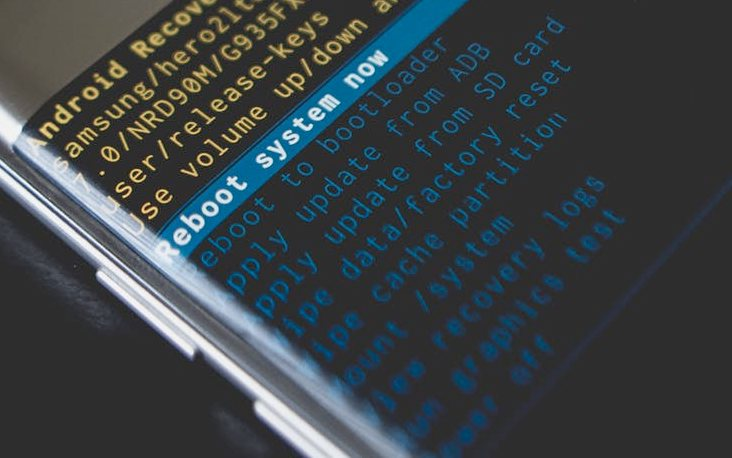
\includegraphics[width=50mm]{images/challenge23.jpg}
\end{marginfigure}

\noindent Eggcryptor is hiding something from you.

Crack it and get the Easter Egg!

\verb+eggcryptor.apk+ is provided.
\subsection{Show Hint (free)}
\begin{itemize}
\item You don't need to run the app. Just decompile and analyze it.
\end{itemize}


\hypertarget{he21.23-solution}{%
\subsection{HE21.23 Solution}\label{he21.23-solution}}

\noindent The apk can be analysed using a decompiler, we used \verb+jadx-ui+.  What it does:
\begin{itemize} 
    \item There is in entry form to get a PIN, this PIN has to match a regular expression of \verb+[a-z][0-9]{4}+
    \item There is a raw, base64 encoded secret stored as raw.raw.
    \item The PIN and the raw data are passed to a crypto function, that does an AES decryption.
    \item If the PIN is correct, we get a picture of an egg.
\end{itemize}

So we can write a brute forcer for the 26*10'000 possible PINs, using the recovered java source code.

\begin{minted}{java}

package com.company;

import java.io.FileOutputStream;
import java.io.FileWriter;
import java.io.IOException;
import java.nio.file.Files;
import java.nio.file.Paths;
import java.util.Base64;
import java.util.regex.Pattern;
import java.util.Base64;

public class Main {
    final static String alph = "abcdefghijklmnopqrstuvwxyz";
    final static String num  = "0123456789";
    public static void main(String[] args) throws IOException {
        final Pattern p = Pattern.compile("[a-z][0-9]{4}");
        final String filePath = "raw.txt";
        String r;
        r = new String(Files.readAllBytes( Paths.get(filePath) ));
        final byte[] raw = Base64.getDecoder().decode(r);
        FileWriter myWriter = new FileWriter("output.txt");

        for (int ia = 0 ; ia < 26 ; ia++ ) {
            for (int i1 = 0 ; i1 < 10 ; i1++ ) {
                String t1 = "" + alph.charAt(ia) + num.charAt(i1);
                for (int i2 = 0 ; i2 < 10 ; i2++ ) {
                    String t2 = t1 + num.charAt(i2);
                    System.out.println(t2);
                    for (int i3 = 0; i3 < 10; i3++) {
                        String t3 = t2 + num.charAt(i3);
                        for (int i4 = 0; i4 < 10; i4++) {
                            String pin = t3 + num.charAt(i4);
                            if (p.matcher(pin).matches()) {
                                //byte[] d = new byte[0];
                                try {
                                    byte[] d = Crypto.decrypt(pin, r);
                                    myWriter.write(pin + ": ");
                                    myWriter.write(d[1]);
                                    myWriter.write(d[2]);
                                    myWriter.write(d[3]);
                                    myWriter.write("\n"); //, d[2], d[3]);
                                    if( d[1] == 'P' && d[2] == 'N' && d[3] == 'G') {
                                        System.out.println("Found solution for PIN " + pin);
                                        try (FileOutputStream stream = new FileOutputStream(pin + ".png")) {
                                            stream.write(d);
                                        }
                                    }
                                } catch (Exception e) {
                                    //pass; //e.printStackTrace();
                                }
                            } else {
                                System.out.println("String " + pin + " does not match pattern!");
                            }
                        }
                    }
                }
            }
        }
    }
}
\end{minted}

% <string name="egg">NB2HI4DTHIXS653XO4XHS33VOR2WEZJOMNXW2L3XMF2GG2B7OY6XKYRYGJMGEMKDHBXXG===</string>

% <string name="pattern">[a-z][0-9]{4}</string>
For the PIN \verb+g0717+ we get the egg 
\begin{marginfigure}
    
\includegraphics[width=50mm]{ch23/solution23.png}
\end{marginfigure}

... and the flag is \verb+he2021{th3r3s_4_h4ck_4_th4t}+

\subsection{Sidenotes}

Within the apk is also a resource named "egg" that is
base32 encoded and when decoded gives
\url{https://www.youtube.com/watch?v=ub82Xb1C8os}.  But by now we know better
than to click on the link...

Within the Crypto class, there is a class variable named "EGG" with contents
that are repeatedly base64 encoded from the original string "nope".  So another
loose end tied up.

\hypertarget{he21.24}{%
  \section{HE21.24 Taco Cat}
  \label{he21.24}}
\begin{marginfigure}
    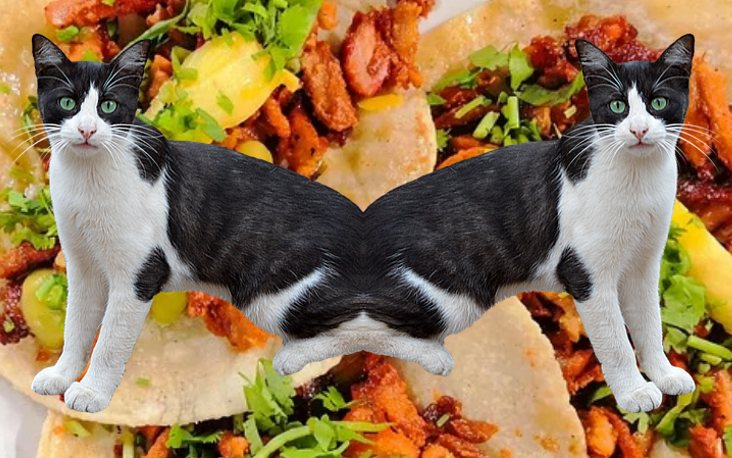
\includegraphics[width=50mm]{images/challenge24.jpg}
\end{marginfigure}

\noindent Was it a cat I saw?

file \verb+tacocat.zip+ provided.

\subsection{Show Hint (free)}
\begin{itemize}
\item lowercase
\end{itemize}

\hypertarget{he21.24-solution}{%
\subsection{HE21.24 Solution}\label{he21.24-solution}}

\noindent 


\hypertarget{he21.25}{%
  \section{HE21.25 Lots of JWTs}
  \label{he21.25}}
\begin{marginfigure}
    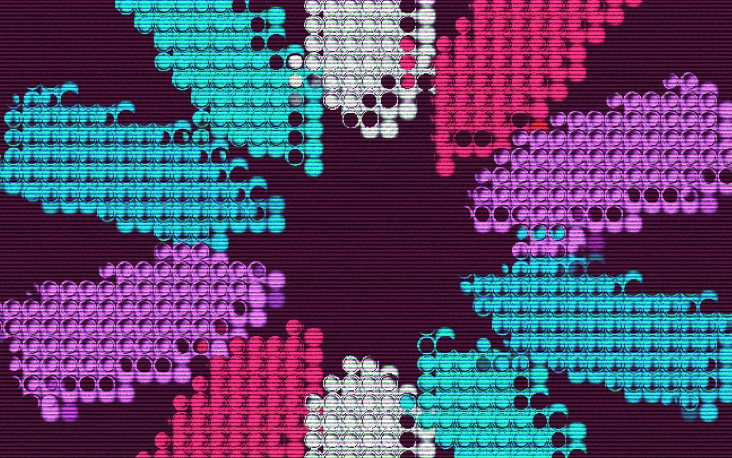
\includegraphics[width=50mm]{images/challenge25.jpg}
\end{marginfigure}

\noindent So many JWTs! What do they hide?

file \verb+jwts.txt+ provided.

\subsection{Show Hint (free)}
\begin{itemize}
\item You better write a script.
\end{itemize}

\hypertarget{he21.25-solution}{%
\subsection{HE21.25 Solution}\label{he21.25-solution}}

\noindent The file contains a jwt that, when expanded, consists again of
several jwts.  Use python to expand them all until we reach the bottom and then
printing the content gives us a list of fragments:

\begin{verbatim}
f_js0
n_t0k
nty_0
he202
1{pl3
k3nZ}
\end{verbatim}

With a bit of imagination these fragments can be combined into
\verb+he2021{pl3nty_0f_js0n_t0kk3nZ}+

\hypertarget{he21.26}{%
  \section{HE21.26 Lost}
  \label{he21.26}}
\begin{marginfigure}
    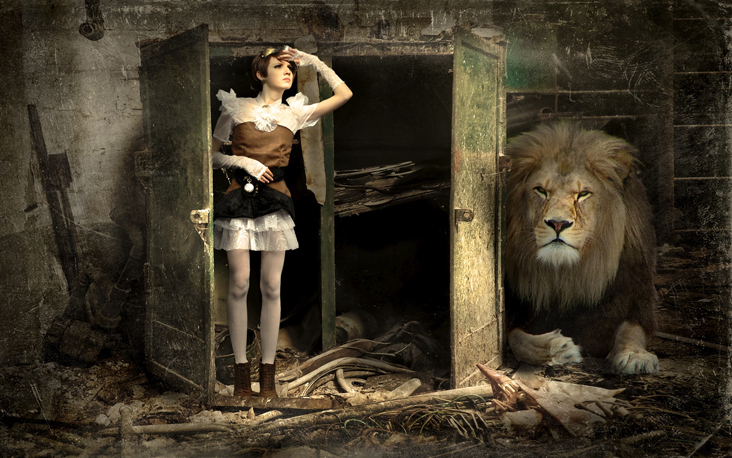
\includegraphics[width=50mm]{images/challenge26.jpg}
\end{marginfigure}

\noindent One of the flags accidentally fell into the pot with the rejected ones!

Can you recover the lost flag?

file \verb+lost.pdf+ provided.

\subsection{Show Hint (free)}
\begin{itemize}
\item 23
\end{itemize}

\hypertarget{he21.26-solution}{%
\subsection{HE21.26 Solution}\label{he21.26-solution}}

\noindent 



\hypertarget{he21.27}{%
  \section{HE21.27 Ghost in a Shell 2}
  \label{he21.27}}
\begin{marginfigure}
    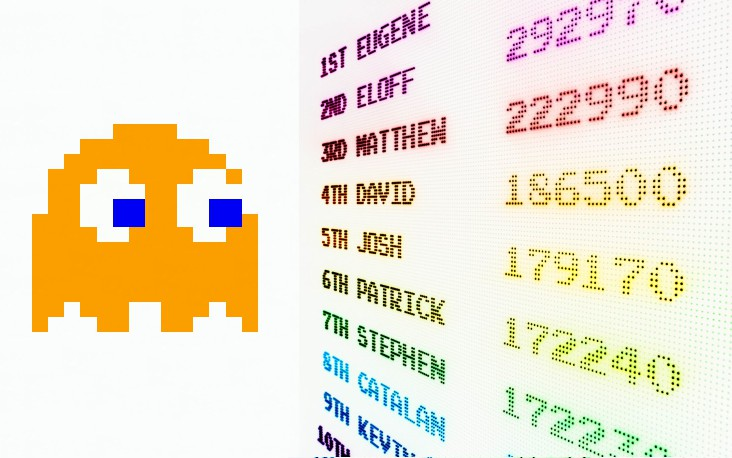
\includegraphics[width=50mm]{images/challenge27.jpg}
\end{marginfigure}

\begin{verbatim} 
  _, _,_  _,  _, ___   _ _, _    _,    _, _,_ __, _,  _,    ,  ,  
 / _ |_| / \ (_   |    | |\ |   /_\   (_  |_| |_  |   |     |  |  
 \ / | | \ / , )  |    | | \|   | |   , ) | | |   | , | ,   |  |  
  ~  ~ ~  ~   ~   ~    ~ ~  ~   ~ ~    ~  ~ ~ ~~~ ~~~ ~~~   ~  ~  
______________________________________________________________________  
 ,--.     ,--.    
| oo |   | oo |   
| ~~ |   | ~~ |   o  o  o  o  o  o  o  o  o  o  o  o  o  o  o  o  o  
|/\/\|   |/\/\|     
______________________________________________________________________  
\end{verbatim} 

\noindent Connect to the server, snoop around, and find the flag!

\verb+ssh 46.101.107.117 -p 2108 -l clyde+
password is: \verb+555-ClYdE+
Note: The service is restarted every hour at x:00.fell into the pot with the rejected ones!

\hypertarget{he21.27-solution}{%
\subsection{HE21.27 Solution}\label{he21.27-solution}}

\noindent 

\hypertarget{he21.28}{%
  \section{HE21.28 Haxxor what 2?}
  \label{he21.28}}
\begin{marginfigure}
    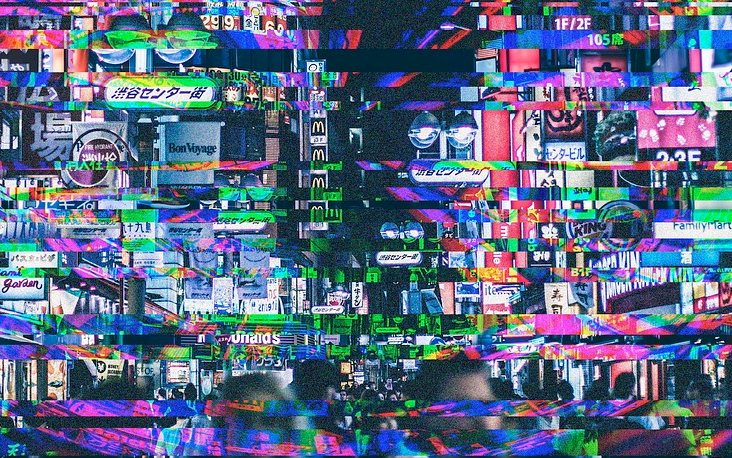
\includegraphics[width=50mm]{images/challenge28.jpg}
\end{marginfigure}

\noindent I was able to break the first file, but I'm stuck at this one.

Help!

file \verb+haxxorwhat2+ provided.

\subsection{Show Hint (free)}
\begin{itemize}
\item This time, the file is not an image.
\end{itemize}

\hypertarget{he21.28-solution}{%
\subsection{HE21.28 Solution}\label{he21.28-solution}}

\noindent 


\hypertarget{he21.29}{%
\section{HE21.29 Sailor's Knot}
  \label{he21.29}}
\begin{marginfigure}
    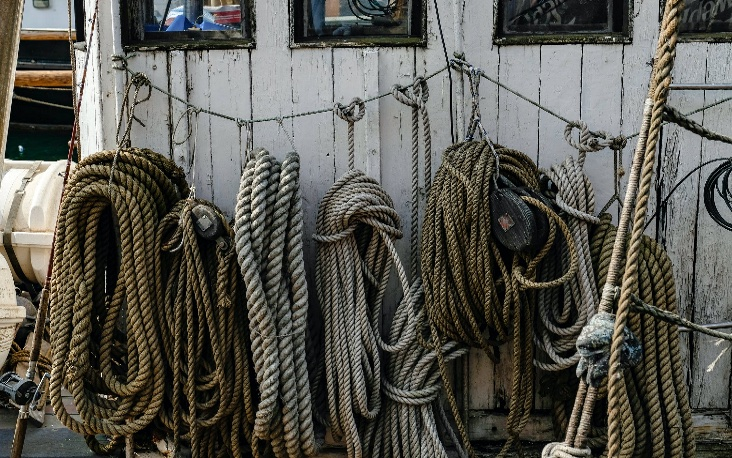
\includegraphics[width=50mm]{images/challenge29.jpg}
\end{marginfigure}

\noindent There is a huge variety of sailor's knots, but the common thing is they all use rops
or other types of cords.

\verb+nc 46.101.107.117 2112+

Get a shell and read the flag.

Note: The service is restarted every hour at x:00

file \verb+sailorsknot+ provided.

\subsection{Show Hint (free)}
\begin{itemize}
\item Ubuntu 18.04 64 Bit
\end{itemize}

\hypertarget{he21.29-solution}{%
\subsection{HE21.29 Solution}\label{he21.29-solution}}

\noindent 



\hypertarget{he21.30}{%
\section{HE21.30 Pix FX}
  \label{he21.30}}
\begin{marginfigure}
    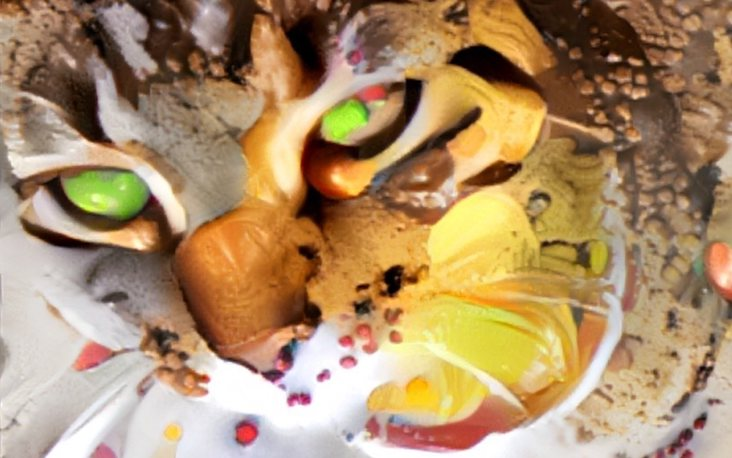
\includegraphics[width=50mm]{images/challenge30.jpg}
\end{marginfigure}

\noindent Hey there! We have our fancy new Pix FX service online!

\noindent Try it out!

\url{http://46.101.107.117:2110}

Note: The service is restarted every hour at x:00

file \verb+sailorsknot+ provided.

\subsection{Show Hint (free)}
\begin{itemize}
\item egg
\end{itemize}

\hypertarget{he21.30-solution}{%
\subsection{HE21.30 Solution}\label{he21.30-solution}}

\noindent 


\hypertarget{he21.31}{%
\section{HE21.31 Hunny Bunny}
  \label{he21.31}}
\begin{marginfigure}
    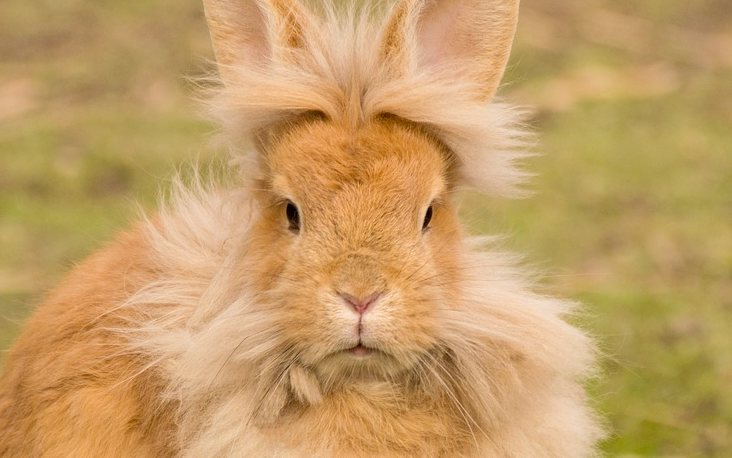
\includegraphics[width=50mm]{images/challenge31.jpg}
\end{marginfigure}

\noindent hunnybunny loves music! Can you figure out what else he loves?

\begin{verbatim}
4ab56415e91e6d5172ee79d9810e30be5da8af18
c19a3ca5251db76b221048ca0a445fc39ba576a0
fdb2c9cd51459c2cc38c92af472f3275f8a6b393
6d586747083fb6b20e099ba962a3f5f457cbaddb
5587adf42a547b141071cedc7f0347955516ae13
\end{verbatim}

⚑ format: \verb+he2021{lowercaseonlynospaces}+

\subsection{Show Hint (free)}
\begin{itemize}
\item The values can be cracked, but they need to be changed somehow first.
\item One of the values represents the flag prefix.
\end{itemize}

\hypertarget{he21.31-solution}{%
\subsection{HE21.31 Solution}\label{he21.31-solution}}

\noindent The lines look like SHA-1 hashes and the hint tells us that one of
them is the prefix of the flag.  So try out the hash of \verb+he2021{+ and
compare it to the given hashes.

The first one is very close

\begin{verbatim} 
input:   4ab56415e91e6d5172ee79d9810e30be5da8af18
he2021{: 4de56415b91b6a5172bb79a9810b30eb5ad8dc18
\end{verbatim} 

From comparison, we see that the characters have been exchanged, `a' with `d',
`b' with `e', and `c' with `f'.  So map the given strings using this rule and
use \verb+hashcat+ to crack the hashes.  From the flag-format, we can limit the
search to lower case letters only, except that for the last part we know that
it has to be terminated with a '\}'.  But first let's try if Crackstation finds
the hashes -- it does!

\begin{verbatim} 
4de56415b91b6a5172bb79a9810b30eb5ad8dc18:he2021{
f19d3fd5251ae76e221048fd0d445cf39ed576d0:hunnybunny
cae2f9fa51459f2ff38f92dc472c3275c8d6e393:ilovemum
6a586747083ce6e20b099ed962d3c5c457fedaae:somuch
5587dac42d547e141071fbaf7c0347955516db13:!}
\end{verbatim} 

The flag is \verb+he2021{hunnybunnyilovemumsomuch!}+

\hypertarget{he21.32}{%
\section{HE21.32 Two Yolks}
  \label{he21.32}}
\begin{marginfigure}
    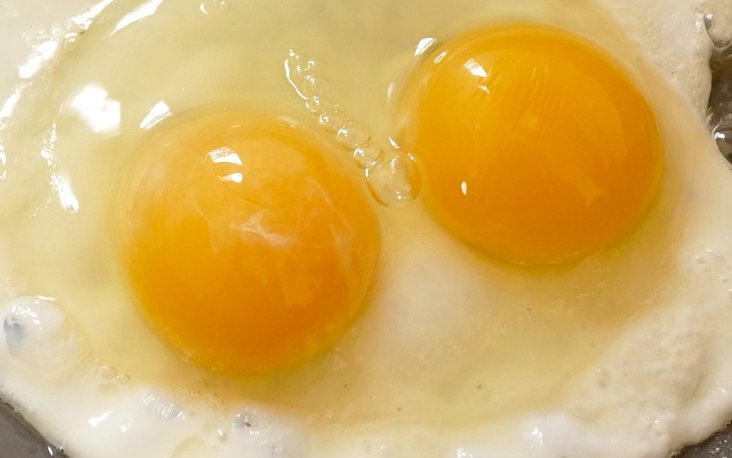
\includegraphics[width=50mm]{images/challenge32.jpg}
\end{marginfigure}

\noindent This egg has two yolks.

But the second seems to be hidden somehow.

File \verb+twoyolks.png+ provided.

\hypertarget{he21.32-solution}{%
\subsection{HE21.32 Solution}\label{he21.32-solution}}

\noindent First step is to analyse the file using binwalk; it reveals that
there are two image contents stored in the file and we probably only see the
first.  Have a look at the bitmaps extracted using \verb+binwalk -e+, we see
that they have both the same number of pixels (1025*1024).  This is consistent
with the size reported in the header of the file.

The first try: try to use \verb+dd+ to copy the second bitmap to the front and
show the image.  It shows then part of the QR-code, but in funky colours and
the bottom is blank.  So analyse the colour indexes used in the bitmaps and we
see that the second bitmap uses a range larger than the palette!  To see if it
contains all of the QR-code, print the bitmaps as ASCII, shifting the values up
by 32 to make them prinable.  It turns out, that the black parts of the QR-code
has all the same value and so we just turn this into a picture using PIL.

\begin{minted}{python}
import png
from PIL import Image

def hist(anArr):
    pal = {}
    for i in range(1025*1024):
        c = anArr[i]
        if c in pal:
            pal[c] += 1
        else:
            pal[c] = 1

    return pal


def saveAscii(fn, arr):
    with open(fn, 'w') as outF:
        for rows in range(1024):
            row = ''
            for cols in range(1, 1025):
                row += chr(arr[rows*1025+cols] + 32)
            outF.write(row + '\n')

with open('pic1', 'rb') as firstF:
    arr1 = firstF.read()
    pal1 = hist(arr1)

with open('pic2', 'rb') as firstF:
    arr2 = firstF.read()
    pal2 = hist(arr2)
    saveAscii('pic2.txt', arr2)

with open('twoyolks.png', 'rb') as pngF:
    r = png.Reader(pngF)
    (width, height, rows, info) = r.read()
    print(info)

print('number of colours in palette:', len(info['palette']))
print('colours used in picture 1:')
for k in sorted(pal1.keys()):
    print('key %d: %d' % (k, pal1[k]))
print('colours used in picture 2:')
for k in sorted(pal2.keys()):
    print('key %d: %d' % (k, pal2[k]))


qr = Image.new('1', (1024,1024))
for rows in range(1024):
    for cols in range(1, 1025):
        p = arr2[rows*1025+cols]
        if p == 15:
            qr.putpixel((cols-1, rows), 0)
        else:
            qr.putpixel((cols-1, rows), 1)
qr.save('qr.png')
\end{minted} 

\begin{marginfigure}
    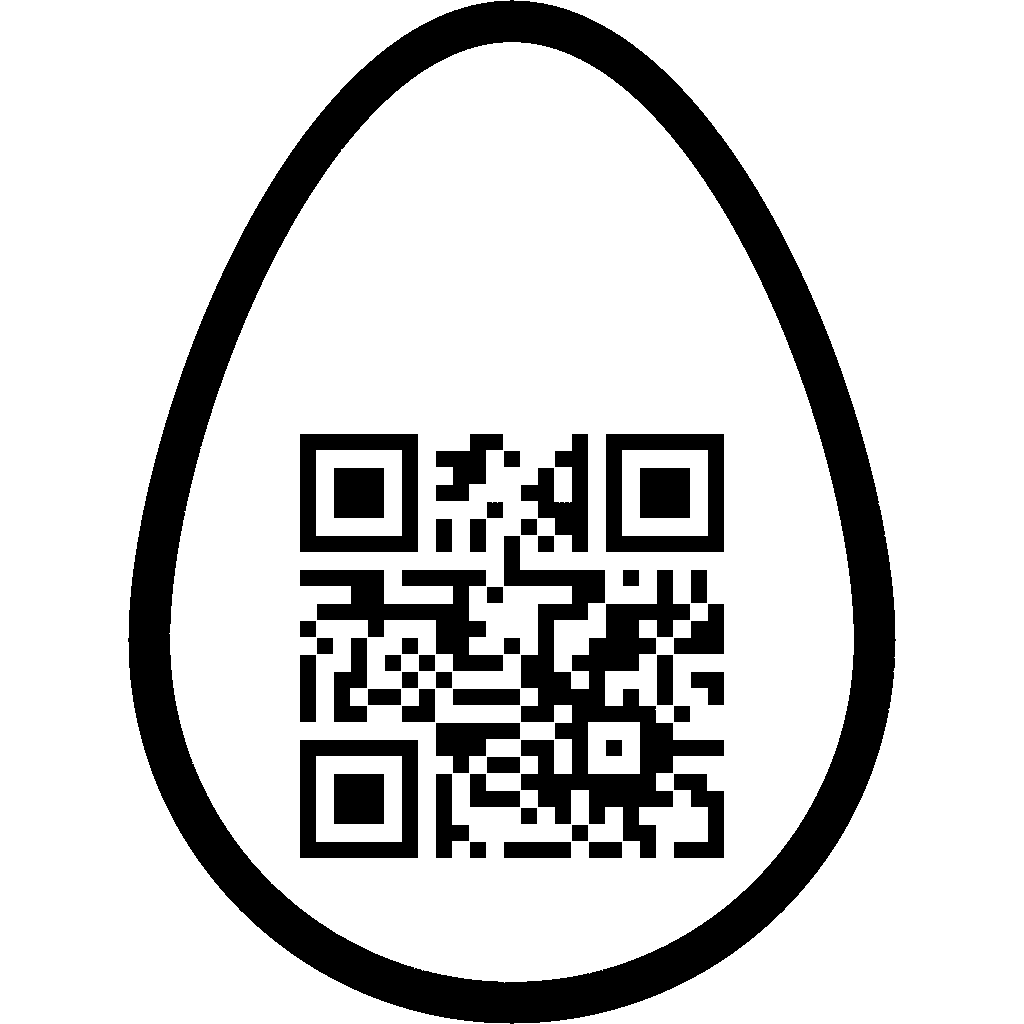
\includegraphics[width=50mm]{ch32/qr.png}
\end{marginfigure}

The flag is \verb+he2021{tw0_y0lks_are_gre33eat}+
\end{document}
